\chapter{\label{ch:1-state_of_the_art}State of the art}

Since the mid-1990s, museums, universities, institutes, and various other types of entities connected to contemporary art have been promoting initiatives aimed at conserving live media art, which has posed significant challenges to traditional conservation practices. These initiatives emerged from the urgent need to find new solutions new solutions to keep this complex and ephemeral art form alive in the future. As a result, traditional conservation paradigms have been fundamentally reshaped, giving way to new conceptual frameworks that have laid the foundation for innovative strategies, including preservation methodologies and documentation models.\\
To date, hundreds of such initiatives have been launched—some of which are still active—and new ones continue to emerge. The problem of conserving live media art remains open and perhaps it can never or should never be definitively closed. However, we are beginning to see shared principles and tools across these initiatives that warrant detailed analysis. Indeed, certain common factors have emerged which, while not officially standardised, have become widely accepted as fundamental to the conservation of this form of art.\\
This chapter aims to highlight the contributions of the many initiatives developed to date, with the goal of identifying the element currently at the core of new conservation strategies. The term ``initiative'' will be used here to focus on the activities that promote research into new conservation strategies. These activities can take various forms, such as projects, networks, working or research groups, and online or physical archives.\\
To conduct this study, we carried out an experimental type of literature review—not based on traditional publications but rather on the activities carried out on the web by these initiatives. The web has become the primary tool that initiatives use to disseminate their research, though it comes with its own challenges. Therefore, this review could more accurately be called ``web-based review.'' Through this review, we will examine both the quantitative and qualitative aspects of live media art conservation to define the state of the art—the current documentation, archiving, and conservation practices implemented by the entities involved.\\
It is important to note that this chapter will not delve into the theoretical and conceptual aspects of these practices, although some references will be made. The focus here is on analysing the practical aspects of conservation. The theoretical framework that underpins this topic will be explored in the next chapter, where we will outline the origins of these practical approaches as well as contemporary perspectives that have yet to be fully integrated into practice.\\
This order of presentation was chosen because, although the practical and theoretical research areas are closely interconnected, the latter has advanced significantly. Chapter~\ref{ch:3-mata-models_and_visual_language} will define the computational model presented in this text based on these theoretical advancements.

\section{Methodology}
The subject area and resources must be clearly defined at the foundation of any literature review. As Rowley and Slack \cite{rowley2004conducting} explain, ``\textit{A literature review distills the existing literature in a subject field; the objective of the literature review is to summarize the state of the art in that subject field.}” However, due to terminological confusion, identifying a central subject in the practice of live media art conservation is challenging. This confusion significantly impacts the review process and serves as a crucial analysis element in the review itself.\\
In order to avoid this terminological confusion in this thesis, we chose to use the term live media art. However, some more common terms are ``time-based media'', ``media art,'' ``new media art,'' ``multimedia art,'' or more specific terms like ``digital art,'' ``installation art,'' or ``performance art.'' While these terms sometimes fully encompass the characteristics of current research (as described in the introduction), they are often only partially relevant. For example, ``performance art'' does not necessarily include technology-based works. Problems arise when terms are misused. For instance, ``multimedia'' is often applied in the digital art context but refers to the simultaneous use of multiple media (both analogue and digital) within an artwork \cite{friedman2023intermedia}. Similarly, ``time-based media art'' is frequently associated solely with video art, but as Laurenson \cite{laurenson2001developing} states, it includes any media that creates a time-based experience. This terminological inconsistency limits control during the review’s search phase, resulting in generic or inconsistent keywords and, consequently, unclear and noisy results.\\
Another significant challenge is the type of resources being studied. Since the goal is to analyse practical outcomes from initiatives such as projects, networks, and archives, traditional resources like papers and books are not the main focus. Instead, web-based resources—websites, web pages, and online posts—are more relevant. Scholars widely use these platforms to share findings and initiatives related to live media art conservation.\\
This shift to web-based resources has both advantages and disadvantages. On the positive side, websites are more open and accessible to a broad audience compared to articles or books. They also allow for the inclusion of diverse materials, particularly multimedia, which can be viewed directly on the site or downloaded. However, the use of web platforms has significant drawbacks, primarily related to maintenance. Maintaining a website requires ongoing effort, both in terms of work, as it needs regular updates and upgrades, and costs. Consequently, websites are more susceptible to the obsolescence of information due to a lack of updates or expired domains—a problem also addressed later in this review.

\subsection{Review platforms}
The resources analysed regarding initiatives of live media art conservation were collected starting from two online platforms: \textit{Monoskop} and the \textit{International Network for the Conservation of Contemporary Art} (INCCA).
\begin{itemize}
    \item The \textit{Monoskop} website is a research platform for the arts, culture, and humanities. It presents wiki pages of contemporary themes and movements in art, culture, and society. Although \textit{Monosko} mainly focuses on the arts and artists, it is also a good search engine for live media art conservation initiatives. More importantly, it already presents a collection of resources on preserving and curating modern and contemporary art. The page (at the link \url{https://monoskop.org/Art/Care}) grew out of a collaborative effort within the \textit{New Approach in the Conservation of Contemporary Art} (NACCA) research network (last updated 24 November 2024). It is a handy starting point for a review of the state of the art.
    \item The \textit{International Network for the Conservation of Contemporary Art} (INCCA) website is a sharing platform for professionals connected to the conservation of modern and contemporary art (conservators, curators, scientists, registrars, archivists, art historians, artists, educators, students, etc.). The website is an ideal space to share the outputs of projects, organised initiatives, open calls, new archives, articles, and interviews within this field. Each INCCA member can share their posts, which are usually formatted with a presentation of the topic and one or more links to other web pages on which the subject is treated and presented in detail. The INCCA website showcases modern and contemporary art conservation initiatives and, thus, is a direct portal toward the websites of museums, archives, foundations, universities, and networks. 
\end{itemize}

\subsection{Review process}
\subsubsection*{Monoskop}
The review process started from \textit{Monoskop}’s resources collection webpage mentioned above. This page presents many lists of resources divided into several sections, such as ``Labs, initiatives, associations,'' ``Publications,'' ``Bulletins, newsletters,'' ``Films,'' ``Research projects, networks, consortiums,'' ``Events,'' ``Exhibitions,'' ``Software tools.'' Only the ``Labs, initiatives, associations'' and ``Research projects, networks, consortiums'' have been considered for the review, with a total of 130 entries. Because of the terminological confusion (many items were strictly related to analogue video preservation and digitalisation, and others were related to fine art), some entries of the lists were deleted, obtaining a total of 65 entries for the \textit{Monoskop} website.

\subsubsection*{INCCA}
The procedures for extracting resources from the INCCA search engine have been more elaborate. We initially collected posts related to conservation practices using seven keywords: \textit{Document}, \textit{Archiv}, \textit{Preserv}, \textit{Conserv}, \textit{Restor}, \textit{Reactivat}, and \textit{Collect}
\footnote{Only the main part of the word is considered, taking into account both the noun, the verb and the gerund (e.g. \textit{Preserv} stands for \textit{preservation}, \textit{preserve} and \textit{preserving}.)
}.
 For each keyword, the search engine results from 6 (in the case of \textit{Reactivat}) to over 1500 posts (in the case of \textit{Conserv}), with a mean of 450 posts for each research and a total of 6304 collected posts. However, many posts overlap with each research.\\
For this reason, we developed a custom web scraper software in Python, which has been used to improve the website search and automatically remove overlaps and extract essential data (posts’ links, publication date, and authors)\footnote{Web scraping software is a tool used to automatically extract data from websites. In our case, the software scanned all the results for each keyword used in the research, identified overlaps, and created a table with the necessary data extracted from the INCCA posts, including the post links, publication dates, and authors. It is a very simple tool that merely speed up the data extraction process. The web scraper application developed for this thesis can be found in the main GitHub repository of this thesis, at the link \url{https://github.com/alessandrofiordelmondo/phd-keeping_live_media_art_alive/tree/master/tools/python-webscrap}}. With this software, we collected 1092 posts. Each collected post was quickly analysed to verify the coherence with the main topic, deleting all the posts referring to other fields such as fine art, photography, and sculpture (as we have done with the \textit{Monoskop} list). We could also classify each post based on its function during this step. We defined five different classes: \textit{Entity} (presentation of an organisation, museum, project, and archive), \textit{Event} (invitation to a conference, summit, symposium, and exhibition), \textit{Publication} (when sharing and presenting books, articles, or theses), \textit{Program} (promotion of a University or organisation study program), \textit{Call} (call for participation to a conference or a publication), \textit{Other} (a miscellaneous of other and unclassified post). Every \textit{Entity} (organisation, university, museum, project, and archive) mentioned in the collected posts was further explored through Google search, allowing the collection of many other projects never mentioned in INCCA. Many entity's websites include sections usually named ``projects'' or ``research''; others have sections dedicated to external resources (e.g. as the ``other research project'' on the DOCAM website or the ``external resources'' page on the \textit{Matters in Media Art} website which allow discovering external resources). The expanded research enables the collection of 76 total entities.\\
The complete collection results in 113 entries, 28 of which overlap between the \textit{Monoskop} and INCCA research procedures.\\
\newline
Each entry has been studied to obtain general information and specifications about the initiative’s objective, goals, and produced outcomes. The in-depth analysis starts from the ``home'' and ``about'' pages of the relative web resources (if present) and continues with reports and published articles. The research aims to extract specific information such as the typology of the initiative, used terminology, developed and utilised methodologies and strategies, and general ones regarding the period and geographical area of activity and founders. Some projects were particularly highlighted for their contribution and the relevance of their produced output.

The research results consist of two tables. The first table contains 113 entries for all the projects. The second table comprises 315 entries and represents the organisations (such as museums, universities, foundations, and many others) that fund, support, or run the initiatives. The table allows for studying the initiatives' geographical spread and the types of organisations involved. The entire tables can be found in Appendix~\ref{ax:e-table_of_initiatives} and Appendix~\ref{ax:f-table_of_organisations}.

%%%%%%%%%%%%%%%%%%%%%%%%%%%%%%%%
%%%%%%%%%%%%%%%%%%%%%%%% RESULTS
%%%%%%%%%%%%%%%%%%%%%%%%%%%%%%%%

\section{Results}
The collected data will be analysed in the following pages. The first section will be a quantitative analysis, taking the most superficial data, referring to the used terminology, period of activity, geolocalisation, and organisations participating in initiatives. The second section will deal with an in-depth and qualitative analysis, considering and comparing the theoretical backgrounds and produced outcomes. 

%%%%%%%%%%%%%%%%%%%%%%%% QUALITATIVE ANALYSIS

\subsection{Quantitative analysis}

\subsubsection{Web platforms}
A first analysis of the web platform where the review was conducted must be done. As mentioned above, the web is the main form of communication and information used by initiatives. Many initiatives’ web spaces reside within the websites of the leading responsible organisations (e.g., almost all the Tate initiatives have their own web space on the museum's website). Other projects, often those bigger and with a larger consortium, have their own website (e.g. the project \textit{Inside Installation}). Finally, some initiatives do not have a website and use other means of information and communication (e.g., the Italian project \textit{Into Installation}, which published its book at the end of the project). Considering all 113 entries, table~\ref{tab:web_plaforma_for_initiatives} summarises the presence of main or sub-web spaces and the lack of web pages.

\begin{table}[!h]
\centering
\begin{adjustbox}{max width=\textwidth}
\begin{tabular}{|l|l|l|} \hline
Main Web space & Sub Web space & No Web space \\\hline
48             & 51            & 14           \\\hline
\end{tabular}
\end{adjustbox}
\caption{\label{tab:web_plaforma_for_initiatives}Web platform for initiatives.}
\end{table}

As already mentioned, the problem with the web is the maintenance, and some resources are unavailable today (12 websites are completely unavailable today). Sometimes, even if the web space is apparently working, it contains death links and no longer available subpages (e.g. the\textit{ Obsolete Equipment} project within scart.be’s website, the \textit{Resurrection Lab} project within the iMAIL’s website and many others). Sometimes, the web space contains just a general description of the initiatives without other information (e.g. the Hallwall Contemporary Art Center’s \textit{Migrating Media} project, the Imai’s \textit{Concretions of the Ephemeral} project and so on).

\subsubsection{Terminology}
In order to conduct a terminological analysis, we measured the popularity of terms initiatives used to refer to art. For those initiatives with available websites, we extracted the terms from the presentation web page (usually in the ``home'' or ``about'' pages of the website). For those initiatives with unavailable websites, we used the \textit{Wayback Machine} provided by \url{https://web.archive.org} \footnote{The \textit{Wayback Machine} at \url{https://web.archive.org} is a digital archive of the internet managed by the Internet Archive, a nonprofit organization. It allows users to access archived versions of websites, preserving historical snapshots of web pages over time.}, which allowed us to trace almost all the past web sources. For those initiatives without websites, the terms were extracted from the project name and the INCCA post in which the projects were mentioned and collected.\\
We extracted 39 terms (considering that many initiatives define the art with more than one term) and their iterations among all the initiatives. The following list presents all the extracted terms (from the most to the least used):
\begin{multicols}{3}
\begin{itemize}
\item contemporary
\item media
\item digital
\item performance
\item new media
\item video
\item time-based media
\item modern
\item installation
\item electronic
\item audiovisual
\item computer-based
\item conceptual
\item dance
\item virtual reality
\item intermedia
\item variable media
\item single-channel video
\item moving image
\item minimal
\item post-minimal
\item visual
\item live
\item net
\item software-based
\item multimedia
\item immersive media
\item public
\item sound
\item internet
\item interactive
\item augmented reality
\item fluxus
\item computer
\item immersive
\item time-based 
\item fine
\item experimental
\end{itemize}
\end{multicols}

Figure~\ref{fig:c1-terms_popularity} shows the iterations of the terms used at least in more than one initiative.

\begin{figure}
    \centering
    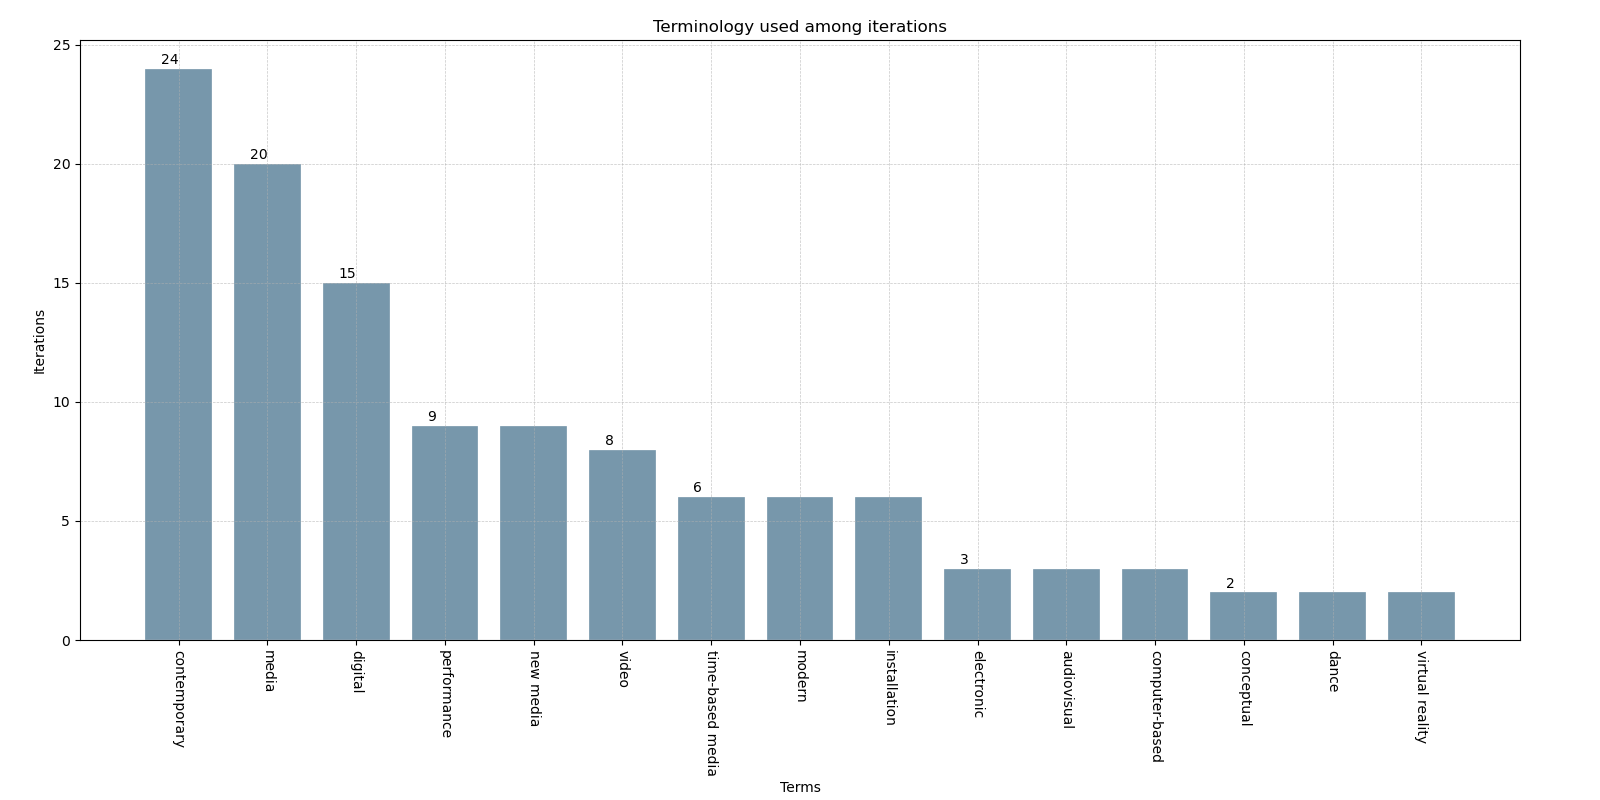
\includegraphics[width=\textwidth]{chapters/1-state_of_the_art/image/plot01-art-terms.png}
    \caption{Popularity of terms initiatives used to refer to art.}
    \label{fig:c1-terms_popularity}
\end{figure}

This data shows that many initiatives use general terms such as ``contemporary'' and ``modern'' art, which are often paired. These initiatives use these terms to embrace different genres and forms. Some examples are SMBK’s \textit{Modern Art: Who Cares?} and \textit{Interview with Artist}, the INCCA network, the web archive \textit{Basis Wien}, and many others. These initiatives include fine art, contemporary sculptures and paintings, as well as technology-based and media art.\\
The term ``media'' is the second most used. However, many initiatives have replaced this term with ``new media'' (with nine iterations) and ``time-based media'' (with six iterations), which are similar and create confusion. It is not straightforward to find a clear distinction between these terms. \textit{Monoskop} has a definition of ``media'' art \footnote{``\textit{The term media art is useful and used for artistic projects bringing up the technological, aesthetical, social, cultural, legal and political issues that come along with the emergence of new media. Since 1990s the new media have included internet, web, mobiles, wireless, GPS, and others. Media culture in this regard uses and is used by new media}” \url{https://monoskop.org/Media_art_and_culture} (last accessed 10/12/2024).}, while it only presents a few articles on ``new media'' art and ``time-based media'' art without a clear definition. Another online resource, such as the \textit{Getty Research Institute's Art \& Architecture Thesaurus}, clearly defines ``new media'' \footnote{``\textit{A genre of art-making practice involved with electronic media such as video, robotics, computer coding, and digital media in general. The term new media has been in use since the 1960s when it was applied to any non-traditional medium, initially video, which then was newly available to artists. With the rapid expansion of digital technologies, the term has come to refer to art that is by its nature electronic or digital and not merely made with with recent technological techniques}” \url{https://www.getty.edu/vow/AATFullDisplay?find=media+art&logic=AND&note=&page=1&subjectid=300435250} (last accessed 10/12/2024).} art and nothing related to ``media'' and ``time-based media'' art. A definition of ``time-based media'' art can only be found in Tate's online glossary Art Terms \footnote{``\textit{Usually time-based media are video, slide, film, audio or computer based. Part of what it means to experience the art is to watch it unfold over time according to the temporal logic of the medium as it is played back}” \url{https://www.tate.org.uk/art/art-terms/t/time-based-media} (last accessed 10/12/2024). Definition that comes from \cite{laurenson2006authenticity}.} (the context in which the term was born), which also presents a very general definition of ``new media'' art but nothing related to ``media'' art. Considering these definitions, it is possible to say that ``media'' and ``new media'' refer to the use of all media (in the Mcluhanian sense of the term) in art - emphasising novelty in the term ``new media''. ``Time-based media'' art adds temporal and processual characteristics to the former terms.\\  
Another interesting term to notice is ``electronic'', which has only three iterations related to two linked initiatives, the V2\_’s \textit{Archive and Capturing unstable Media}, and the \textit{ActiveArchive} archive. We can not find a clear definition of the term in these initiatives or the \textit{Monoskop} and Tate Terms search engines. We can see a short definition in the \textit{Getty Research Institute's Art \& Architecture Thesaurus} \footnote{``\textit{Collective term used to refer to all art works which employ electronic media or technology}” \url{https://www.getty.edu/vow/AATFullDisplay?find=electronic+art&logic=AND&note=&english=N&prev_page=1&subjectid=300387714} (last accessed 10/12/2024).}, which only specifies the electronic character of the media used. For this reason, ``electronic'' art could be juxtaposed to the three previous terms.\\
All the other collected terms refer to specific mediums and forms, such as ``digital'', ``performance'', ``video'', ``installation'', ``computer-based'', ``conceptual'', ``dance'', ``audiovisual'', and ``virtual reality''. These terms highlight the initiatives' research focus but do not elucidate the terminological confusion.

\subsubsection{Timeline}
Another critical data source is the initiation and activity periods of the initiatives, which makes it possible to represent and understand the progress of the initiatives and overall activity related to the studied subject. For this purpose, it was necessary to extract the activity period of each initiative, i.e. to obtain start and end dates. However, while almost all initiatives have a clear timeline, few do not have a clear beginning or end date, leaving much uncertainty about their timeline and progress. For this reason, these initiatives (six) were excluded from the analysis.\\
Figures~\ref{fig:c1-launched} and ~\ref{fig:c1-active} provide two different representations of the initiative's timeline, showing the number of initiatives launched (Figure~\ref{fig:c1-launched}) and the number of active initiatives (Figure~\ref{fig:c1-active}) every year. 

% \begin{figure}
%     \centering
%     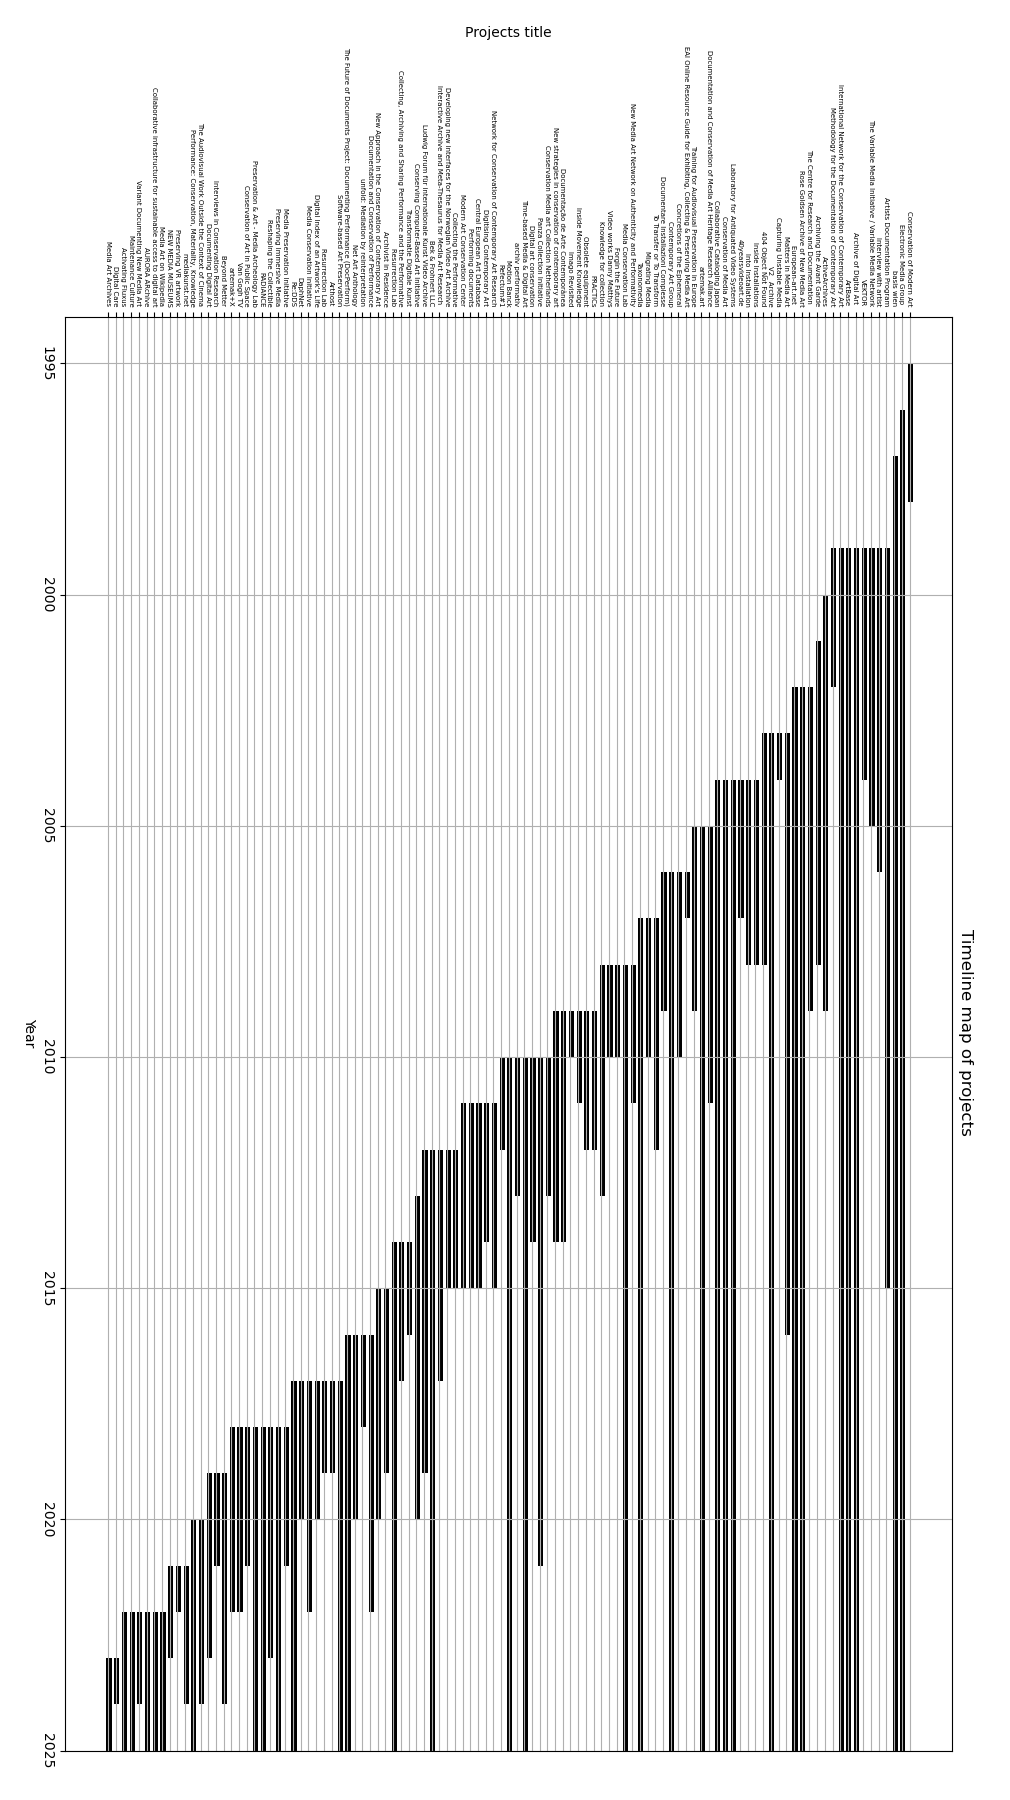
\includegraphics[width=0.9\textwidth]{chapters/1-state_of_the_art/image/plot01-timeline-vertical.png}
%     \caption{Timeline of all the initiatives, starting from 1995.}
%     \label{fig:c1-timeline}
% \end{figure}

\begin{figure}[!h]
    \centering
    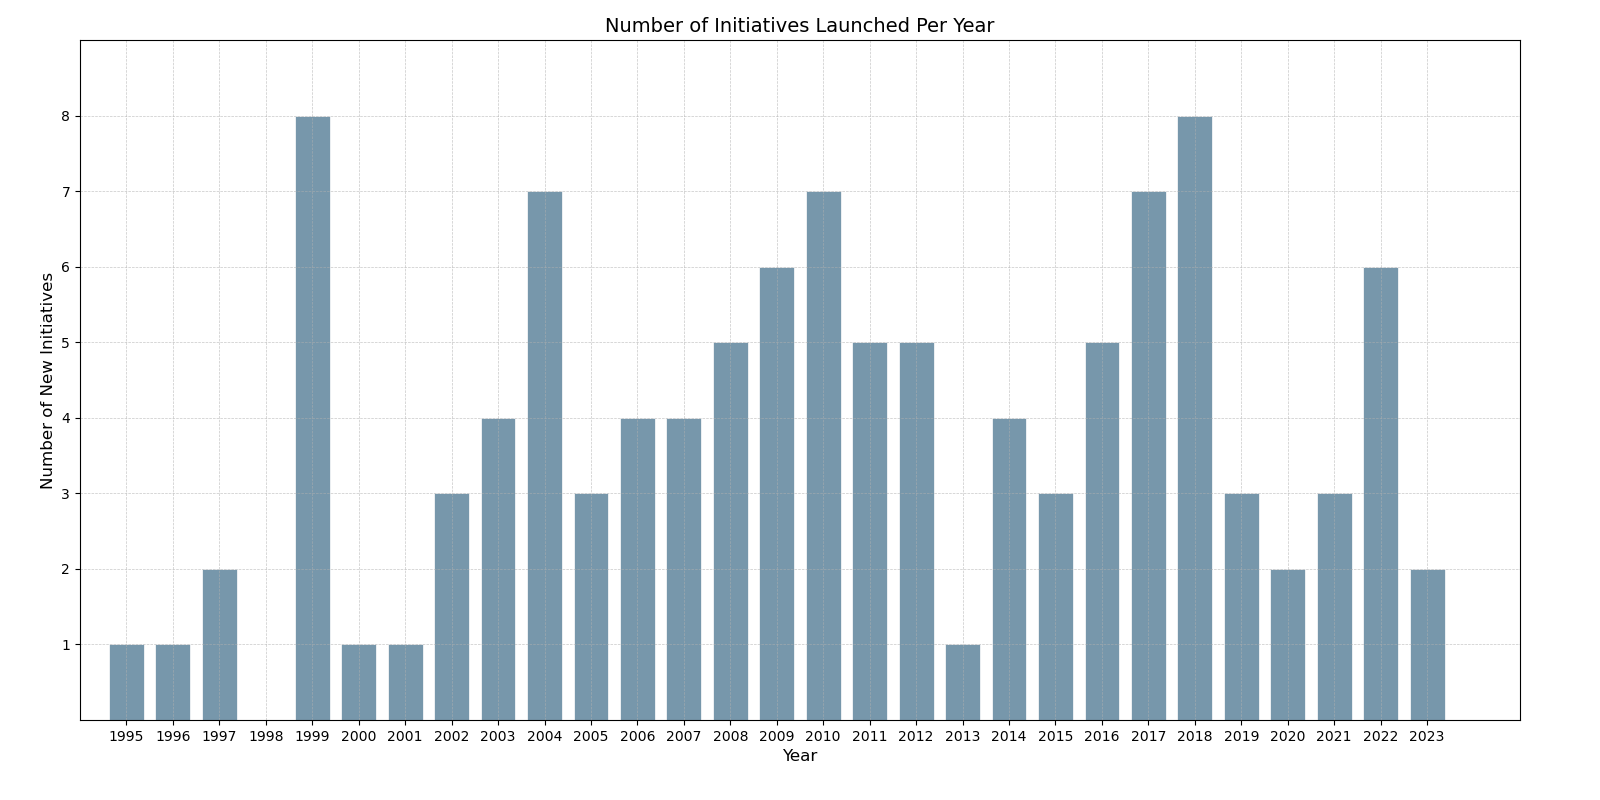
\includegraphics[width=\textwidth]{chapters/1-state_of_the_art/image/plot01-lunchedproject.png}
    \caption{Number of initiatives initiated every year since 1995.}
    \label{fig:c1-launched}
\end{figure}

\begin{figure}[!h]
    \centering
    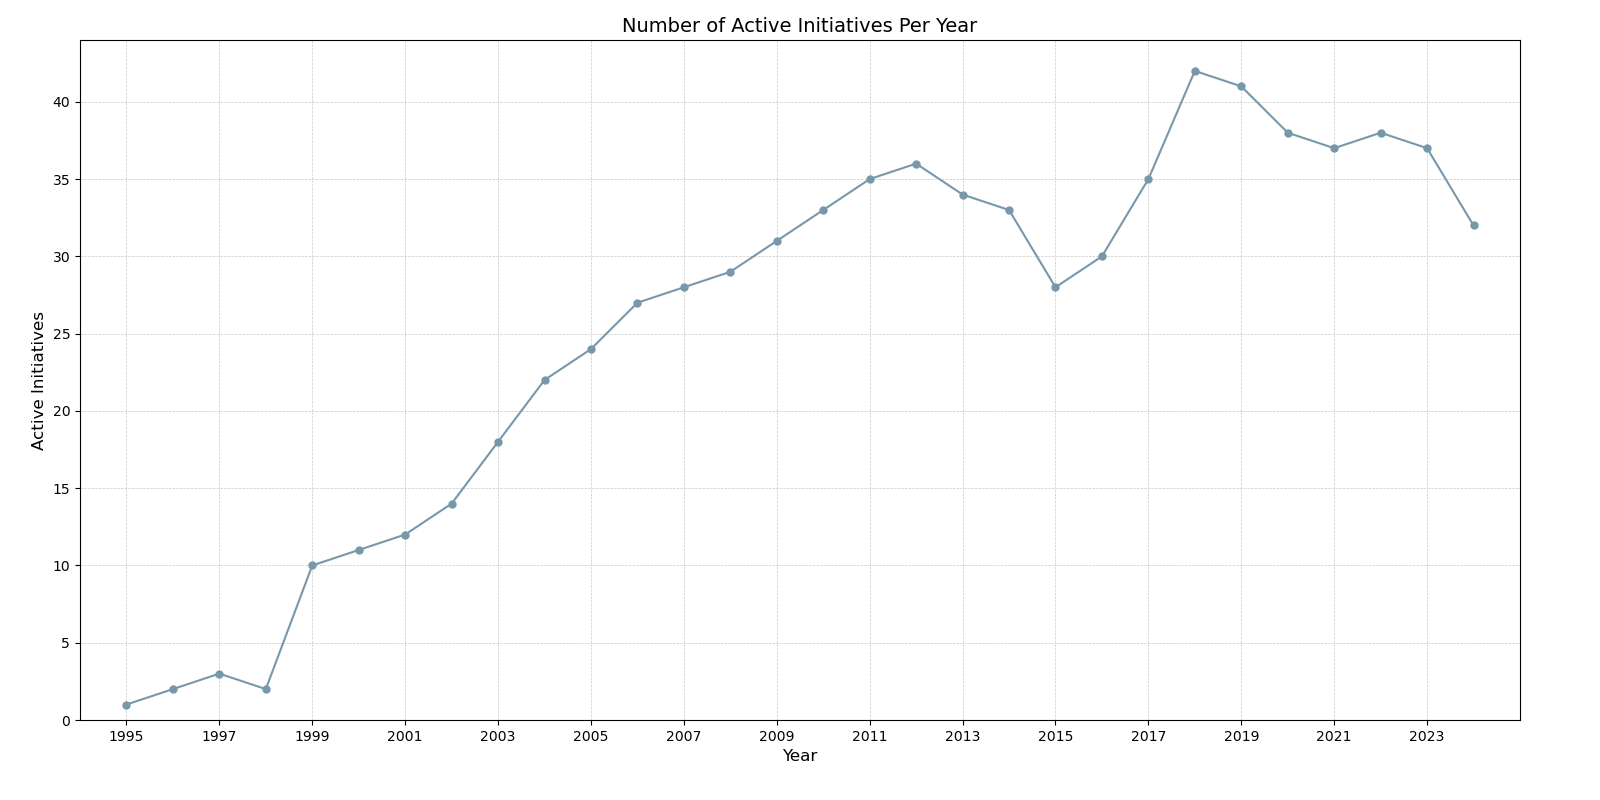
\includegraphics[width=\textwidth]{chapters/1-state_of_the_art/image/plot01-activeproject.png}
    \caption{Number of active initiatives for every year since 1995.}
    \label{fig:c1-active}
\end{figure}

Important information that we can extract from these data is the beginning of the research activity in this subject field, which started in 1995 with the well-known SBMK three-year project \textit{Conservation of Modern Art / Modern Art: Who Cares?}.\\
It is not possible to read a specific behaviour in initiative initiation (Figure~\ref{fig:c1-launched}), be it constant, increasing, or decreasing. However, we can observe some peaks in initiative initiation, especially in 1999 and 2018.\\ 
Figure~\ref{fig:c1-active} shows the overall activity in the subject field. Since its beginning in 1995, it has increased over the years and reached its maximum peak in 2018 (with 41 initiatives active in the field).\\
Another interesting data point that we can extract from the timeline representation is the average duration of the initiatives, which is 2.8 years.

\subsubsection{Geographical distribution}
Another critical piece of data collected is the geographical distribution of the initiatives. To analyse this data, we counted the countries of the organisations involved in each initiative, and the results are shown in Figure~\ref{fig:c1-geo}.\\
The first thing to notice is the dominance of projects from Western countries, mainly Europe. This data may reflect both cultural factors and potential bias in the web-based review itself. Although the INCCA network includes non-Western regional groups like INCCA Asia Pacific and INCCA Korea, these groups have fewer members and posts than the leading INCCA network. Additionally, in the \textit{Monoskop} sections ``Labs, Initiatives, Associations'' and ``Research Projects, Networks, Consortiums,'' only 4 out of 130 entities are related to non-Western projects.\\
Finally, as shown in Figure~\ref{fig_c1-geo}, the Netherlands is the most active country in this field, resulting in 88 times the total number of projects collected.

\begin{figure}[!h]
    \centering
    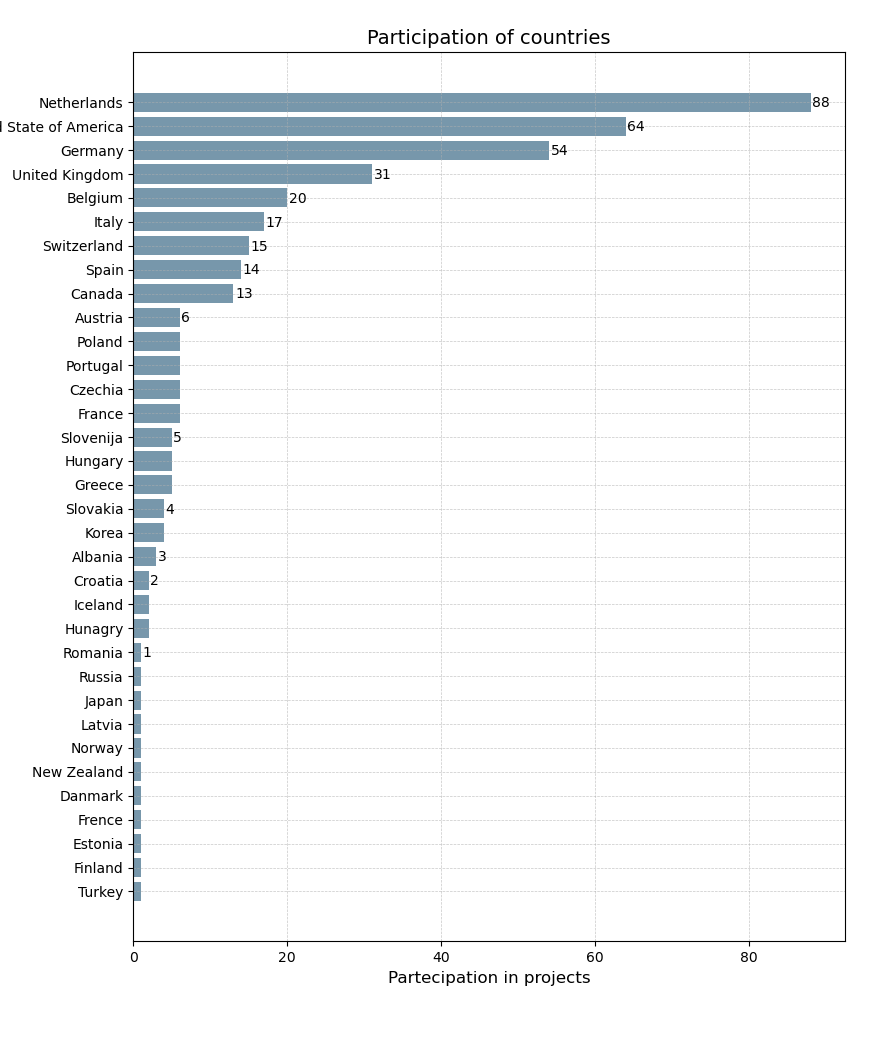
\includegraphics[width=\textwidth]{chapters/1-state_of_the_art/image/plot01-countries.png}
    \caption{Countries’ participation in conservation initiatives}
    \label{fig:c1-geo}
\end{figure}

\subsubsection{Organisations}
Related to the previous data, the leading organisations involved and their typologies are also essential pieces of data that help us understand the context in which the initiatives are developed.\\
Figure~\ref{fig:c1-org} shows the leading organisations involved, with at least five participations in different initiatives. These results perfectly reflect the previous one, with a significant prevalence of Netherlands organisations (LIMA, The Foundation for the Preservation of Modern Art, Netherland Media Art Institute, University of Amsterdam, and Cultural Heritage Agency of the Netherlands). However, Tate has the highest number of initiative participations (13).

\begin{figure}[!h]
    \centering
    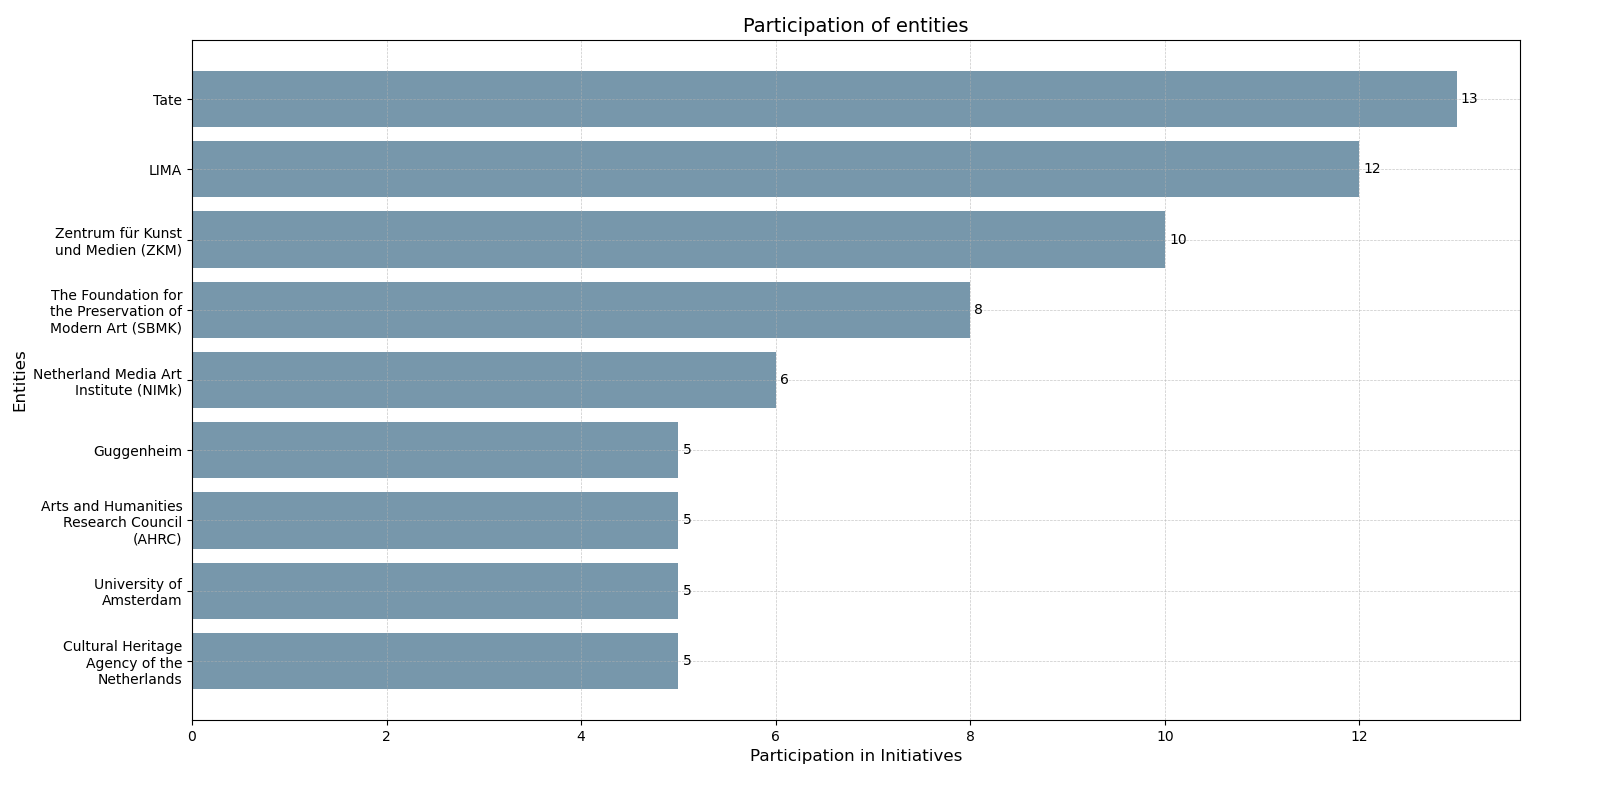
\includegraphics[width=\textwidth]{chapters/1-state_of_the_art/image/plot01-organisation.png}
    \caption{Principal organisation to participate in conservation initiatives}
    \label{fig:c1-org}
\end{figure}

Figure~\ref{fig:c1-org_type} shows the presence of different types of organisations. Although this data is particularly relevant for understanding the initiatives development context, it remains somewhat weak because of the definition of the types listed in the figure. The definition is extracted from the organisation's website on the ``home'' or ``about'' pages.\\
``Museums'' and ``universities'' (including Academies, private schools, University departments, and laboratories) remain the most fixed definitions. This data shows that universities substantially participate in these initiatives, which is interesting and important to consider. Another piece of data extracted from INCCA, although outside the scope of the analysis of initiatives, is the growth of university and academic programs specialising in conserving technology-based arts\footnote{Examples include the \textit{Still Water} program at the University of Maine in Orono, USA, founded by Joline Blais and Jon Ippolito in 2002. This program focuses on New Media art and played a key role in developing the project \textit{Forging the Future: New Tools for Variable Media Preservation}. Another example is the \textit{New Approaches in the Conservation of Contemporary Art} (NACCA) PhD program, coordinated by the Faculty of Arts and Social Sciences at Maastricht University in the Netherlands from 2015 to 2019. Additionally, the \textit{Conservation training program} at the Academy of the Arts in Bern, launched in 2021, specializes in the conservation of modern materials and media.}.\\
Other definitions, such as ``Institutes'', ``Centers'', and ``Foundations'', are more blurred. They sometimes overlap with each other and with completely different definitions, such as Museums.\\
``Institutes'' and ``centres'' are usually overlapped as definitions, so they are joined together. ``Institutes and Centers'' support and advance various aspects of art through activities like research, exhibition, conservation, education, and technology integration. These entities focus on different specialities, such as museum technology, media art, digital culture, cultural heritage, and fine art scholarship. While each institute and centre may concentrate on particular areas, they all contribute to the broader goal of promoting and conserving contemporary arts. Among the most important examples are the Zentrum für Kunst und Medien (ZKM)\footnote{The definition of ZKM given in its website: ``\textit{The ZKM | Center for Art and Media Karlsruhe is a unique cultural institution worldwide, because it is a place that expands the original tasks of the museum [...] In its work, ZKM combines research and production, exhibitions and performances, collections and archives, mediation and events. Through interdisciplinary connections of these fields of work, ZKM as an agile organization can present and produce the development of art and media of the 20th and 21st centuries}'' \url{https://zkm.de/en/about-zkm} (last accessed 10/12/2024).} and LI-MA \footnote{The definition of LI-MA given on its website: ``\textit{LI-MA plays a key role in the future-proof archiving, conservation and distribution of works from the field of media art. LI-MA is a platform for digital art and media art in Amsterdam. With years of experience in conservation and management and as a leading pioneer in the field, LI-MA plays a key role in the future-proof archiving, conservation and distribution of works from the field of media art. Specialist conservation is important to ensure that media and digital art remain accessible in the future despite rapid technological developments. As a knowledge centre, LI-MA is the link between artists, museums, cultural and scientific institutions and the public that engage with visual art and digital culture}'' \url{https://li-ma.nl/article/vision-and-mission/} (last accessed 10/12/2024).}. Sometimes, institutes and centres can own their collection and exhibition space, such as the Instituto Valenciano de Arte Moderno (IVAM) and the House of Electronic Art (HEK). The last one also defines itself as an ``interdisciplinary museum''.\\
The ``Foundation'' is another blurred and broad term. We define a ``Foundation'' as a non-profit organisation established to support charitable, educational, cultural, or other public interest activities. In the context of this specific research field, foundations usually provide grants to initiatives. Among the most important foundations are the Mellon Foundation—which founded many relevant projects such as the \textit{Artist Documentation Program} and \textit{Reshaping the Collectable}—and the Franklin Furnace Foundation—which founded projects such as \textit{The Variable Media Initiative}.\\
Another term is ``Company'', which refers to private companies focused on technologies, software, and informatic system development, such as Ubitech and FT Design Lab, and private companies specifically focused on preserving contemporary art, such as Bek \& Frohnert LLC.\\
Other voices listed in the figure are ``Government Ministries'' - support, funds, and promote initiatives-, ``Physical Archives'', ``Galleries'', ``National Institutes'' - government institutes, usually ministerial ones, specialising in cultural heritage - ``Networks'', ``Collections'', ``Miscellaneous'' - non-profit organisations not well-defined and with an extensive range of activities, such as Rhizome, Voica in Contemporary Art (VoCA), Independent Media Arts Preservation (IMAP), In Between Time (IBT) -, and ``Festival''. Other less common typologies include ``Journal'', ``Library'', ``Association'', ``Auction house'', etc. (refer to Appendix~\ref{ax:f-table_of_organisations}).

\begin{figure}[!h]
    \centering
    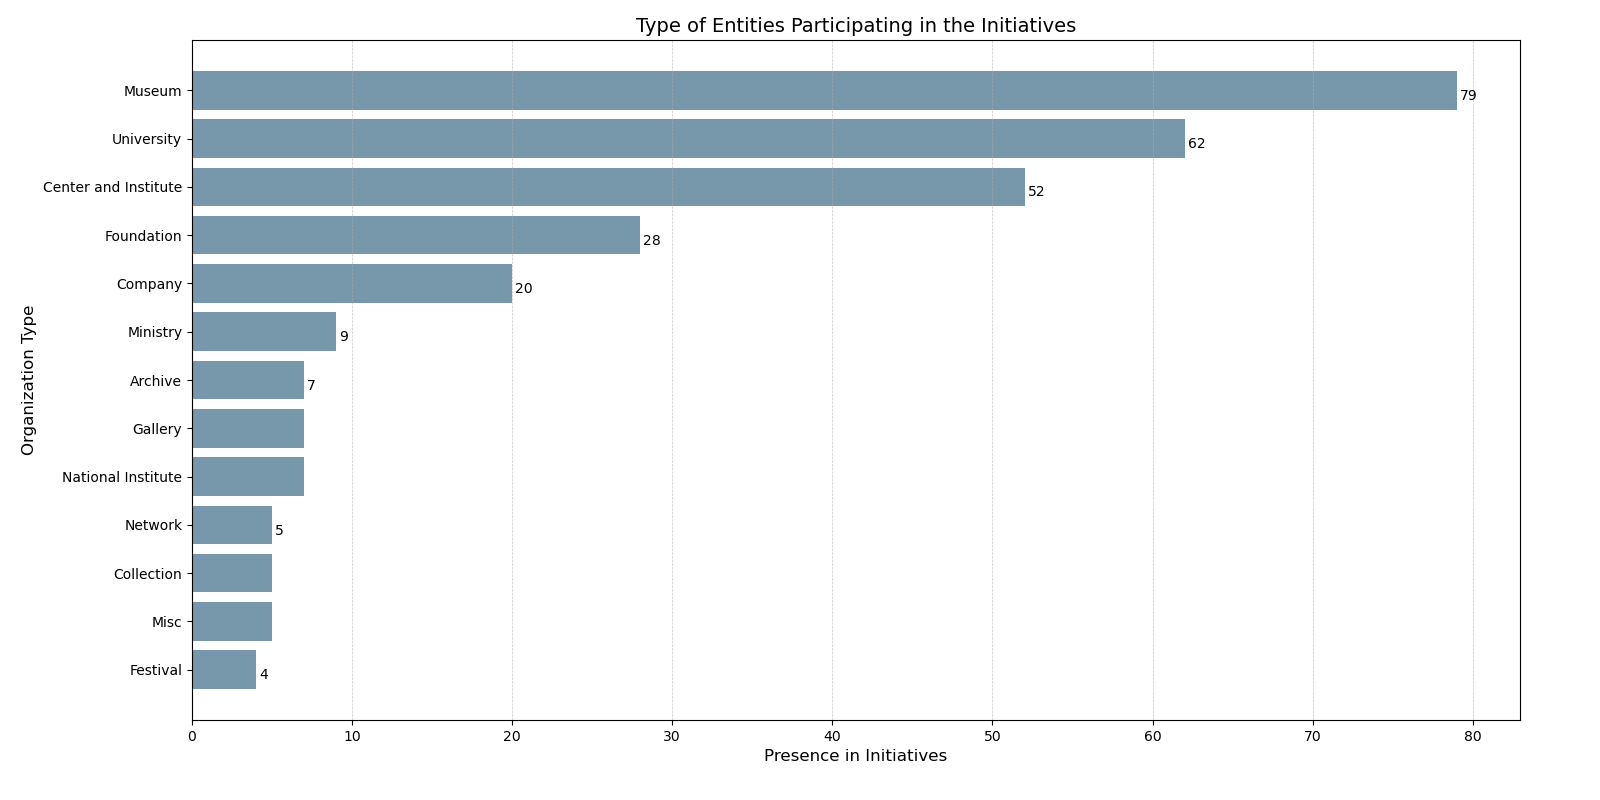
\includegraphics[width=\textwidth]{chapters/1-state_of_the_art/image/plot01-orgtypes.png}
    \caption{Participation of different types of organisation}
    \label{fig:c1-org_type}
\end{figure}

%%%%%%%%%%%%%%%%%%%%%%%% QUALITATIVE ANALYSIS

\subsection{Qualitative analysis}
Given a first quantitative overview of the initiative, a qualitative analysis involves a thematic, non-numerical, and comprehensive review of all the entries. It includes a full exploration of the website and all the resources (articles, videos, blogs, podcasts, etc.) related to each initiative.\\
As evident from the analysis below, there will be some over-mentioned initiatives. The reason is the relevant contributions and outcomes and the readily available, clear and comprehensive documentation of these initiatives. These initiatives include the \textit{Variable Media Initiative}, \textit{Matters in Media Art}, \textit{Capturing Unstable Media}, \textit{Inside Installation}, DOCAM, the \textit{EAI Online Resource Guide}, \textit{Media Conservation Lab}, \textit{Time-based Media \& Digital Art}, \textit{Media Conservation Initiative} and \textit{Media Preservation Initiative}. They present comprehensive information about the initiative and its outcomes, as well as working and intuitive websites and available external resources. Thanks to these initiatives, it was possible to define the macro thematic areas of the analysis, which were then filled in, characterised and deepened with the information collected by the other initiatives.\\
The main macro-thematic and sub-thematic areas analysed are:
\begin{itemize}
    \item Issues of preserving and documenting time-based media art
    \item Limitations of traditional preservation strategies
    \item New preservation strategies
    \item Documentation
    \begin{itemize}
        \item Documentation process
        \item Identity report
        \item Iteration report
        \item Condition report
        \item Documentation models
        \item Thesaurus and Glossary
        \item Interview
    \end{itemize}
\end{itemize}
\subsubsection{Issues of preserving and documenting time-based media art}
The first analysed macro-thematic area has been the incipit of all these initiatives, namely the challenges of conserving and documenting live media art. All the initiatives are born to find practical or theoretical solutions to specific problems.\\ 
Challenges concerning the preservation of live media art can be divided into distinct and hierarchical classes. These challenges encompass the \textit{creative process}, the \textit{intrinsic} and \textit{extrinsic} features of artworks, and the \textit{derivative issues} of conservation. This subdivision allows us to better describe the problems of conserving and documenting live media art in an organised way.\\
Figure~\ref{fig:c1-issues} provides an overview of the hierarchical structure of these features and issues. \textit{Intrinsic} refers to factors inherent to artworks themselves (physical and contextual) and the experience they produce. \textit{Extrinsic} refers to subsequent consequences, extending beyond the immediate realm of the artwork and its experiential dimensions. The \textit{creative process} refers to the development and production phase of the artwork. Finally, the \textit{derivative issues}—derived from the artwork features–summarise all the problems challenging the preservation of live media art. 

\begin{figure}[!h]
    \centering
    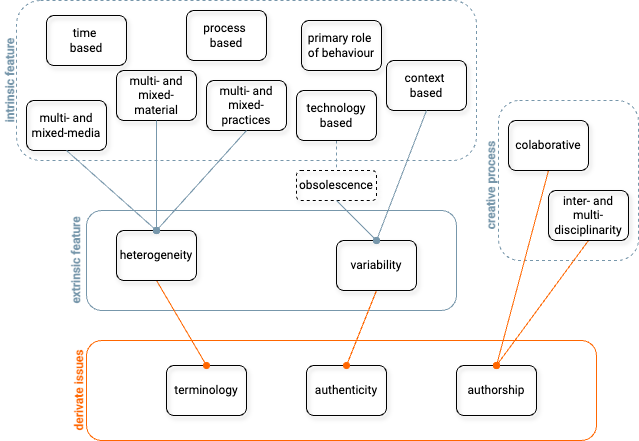
\includegraphics[width=\textwidth]{chapters/1-state_of_the_art/image/graph-issues.png}
    \caption{The diagram represents the \textit{intrinsic}, \textit{extrinsic}, and the \textit{creative process} features of live media artworks and the \textit{derivative issues} related to their preservation.}
    \label{fig:c1-issues}
\end{figure}

\paragraph*{Intrinsic}
The main \textit{intrinsic} features of the artworks considered by the initiative studied are their time and process nature, which classifies them as ephemeral [\textbf{CIAO}, \textbf{Performance conservation}, \textbf{Capturing Unstable Media}]. Both performance and installation exist only when performed or installed, and during their existence time frame, they produce an experience that unfolds over time. For this reason, most initiatives consider live media artworks as \textit{allographic} [\textbf{Guggenheim}], like other art forms such as music, dance and theatre.\\
Live media artworks use a wide variety of materials, tools, methods, and practices often linked and mixed between them and whose significance is unique and inscribed in the individual work [\textbf{Conservation of Modern Art}, \textbf{Capturing Unstable Media}, \textbf{Preserving Immersive Media}, \textbf{CIAO}]. Artworks may be analogue or digital, are often multimedia-based, and contain images and sound that may also be analogue or digital, fixed or moving, pre-existing or directly generated, and so on [\textbf{DOCAM}].\\
They are based on technology and use various devices, usually adapted or created by artists and collaborators. Technologies range from more to less conventional and sometimes cutting-edge ones, and they can include film, video, computers, electromechanics, robotics, web, networking, and so on [\textbf{Inside Installations}, \textbf{DOCAM}, \textbf{EAI}, \textbf{Documentação de Arte Contemporânea}]. The use of technology in artworks is often unconventional, exploring new possibilities, bugs and anomalies [\textbf{EAI}].\\
Another important inherent factor is that live media artworks are often based on the context of the original manifestation. They are usually developed with a specific and strict relationship with the space they occupy and the time of their production. Moving artworks to another context, location, and time can profoundly alter their meaning [\textbf{Capturing Unstable Media}, \textbf{Inside Installation}, \textbf{Documentação de Arte Contemporânea}, \textbf{NeCCAR}]. Especially for performance-based artwork, there is also a strong relation with the original performer(s) (very usually the author) [\textbf{NeCCAR}, \textbf{Collecting the performative}, \textbf{Collecting the performative}].\\
Most importantly, all these artworks show a relevant shift in the creation process, from the object and its physical materiality to the emphasis on the concept [\textbf{Documentação de Arte Contemporânea}] and the primary role of behaviour.\\
The primary role of the artwork’s behaviour, which is the live experience activated by the relationship of the artwork’s presence and the context (including the surrounding space, the moment, and the performers and audiences), seems to be accepted by most initiatives. As one of the first and groundbreaking initiatives in the field, the \textit{Variable Media Initiative} highlights the importance of behaviour, classifying its different forms in art as contained, installed, performed, interactive, reproduced, interchangeable, encoded, and networked [\textbf{Variable Media Initiative}]. The DOCAM research alliance defines behaviours as interactive, processual, procedural, programmatic, distributed, hybrid, migrant, ethereal, collaborative, or a mix [\textbf{DOCAM}].\\
Among these behaviours, which often overlap and whose definitions are usually blurred, the interactivity is mainly highlighted by the initiatives. The ``acclaimed'' interactivity (as defined in the \textit{Capturing Unstable Media}) allows the user to interact with the artwork, manipulate or take home components of a physical work [\textbf{Variable Media Initiative}], and in general and most importantly, allow people to influence input and output and become active participants rather than spectators [\textbf{Capturing Unstable Media}].

\paragraph*{Extrinsic}
All these \textit{intrinsic} characteristics generate \textit{extrinsic} features, which determine the main issues in preserving live media art. We can distinguish two macro-factors: heterogeneity and variability.\\
Contexts, technologies and mixes of material, practices and media are combined in an individual and original way for each artwork. That means every artwork is a world of its own, with its components, appearance and experience. In other words, artworks are heterogeneous, making it difficult to find standard practices and terminologies to describe them. 
On the other hand, variability is a more complex feature that makes the artwork unstable and in a constant transformation process: a transient process rather than a fixed object [\textbf{Methodology for the Documentation of Contemporary Art}, \textbf{DOCAM}]. This variability is primarily the result of context- and technological-based features of artworks.\\
Since each artwork has a relationship with the context (e.g., the surrounding space of a specific location), when it is ``re-presented'' or ``re-interpreted,'' it should be adapted to the circumstances of the new context, appearing differently each time [\textbf{Concretions of the Ephemeral}]. Therefore, each manifestation may be considered a different representation of the artwork [\textbf{CCBA}] or, from another perspective, based on a mutable context [\textbf{EAI}].\\
However, the technological feature of live media art determines the central problematic aspect of variability, which is also the main challenge of most initiatives. Live media artworks suffer from the fragility and ageing of the technologies involved, which are difficult to repair or replace because of the rapidly evolving technological landscape [\textbf{Variable Media Initiative},\textbf{ Capturing Unstable Media}, \textbf{DOCAM}, \textbf{Inside Installations}, \textbf{Obsolete Equipment}, \textbf{ActiveArchives}, \textbf{Concretions of the Ephemeral}, \textbf{Archivist in residence}, \textbf{Software-based art preservation}, \textbf{CCBA}, \textbf{UNFOLD}]. Therefore, like everyday technology such as display equipment, smartphones, computers, and home appliances, even artworks quickly become obsolete. So, to present the artwork again, some components have to be repaired but usually have to be replaced with new technologies that can reproduce the behaviour of the old ones. Although this operation is not always possible, mainly when the meaning and goal of the works lie in their material components [\textbf{DOCAM}], it is still controversial from the perspective of the ethics of traditional restoration [Concretions of the Ephemeral].\\
Finally, the variability of the artworks should also consider perishable [\textbf{Documentação de Arte Contemporânea}], degradable [\textbf{NeCCAR}], and consumable materials.

\paragraph*{Creative process}
Another issue involves the \textit{creative process}. The V2\_’s \textit{Capturing Unstable Media} initiative focuses on this. Instead of viewing artworks as final ``precious originals'' created by a single ``artist's genius,'' we need to consider their ongoing process and ``distributed authorship.'' The \textit{Capturing Unstable Media} initiative suggests calling electronic artworks ``projects'' to reflect this shift. These projects are part of a larger entity or process, including research, development, festivals, and exhibitions. They use various materials and methods and involve interdisciplinary or multidisciplinary collaborations. Projects often do not end after their first showing; they have multiple stages with different people contributing. The results come from a team effort between artists, scientists, engineers, and designers. Together, these teams create artistic and cultural expressions within broader contexts like research themes, performances, and festivals, known as \textit{aR\&D} (artistic Research and Development) [\textbf{Capturing Unstable Media}].

\paragraph*{Derived}
So, considering these \textit{intrinsic} and \textit{extrinsic} features as well as the issues related to the \textit{creative process}, the primary layer of live media art preservation issues arises, which includes the authenticity and the authorship of the artworks.
One of the most theoretical and practical challenges of live media art conservation is the notion of the ``original'' [\textbf{inside installations}] and, therefore, determining the authenticity. The behaviour-based character, the ephemeral nature, and the variability of the art are thrown into crisis by this fundamental notion of ``originality'' that is the basement for conservators, museums, and collectors. What is essential to determine the origins and authenticity of the work? What parts of it should be preserved, transformed or re-created? [\textbf{Inside installation}]\\ 
Another issue concerns the authorship and the artwork's intellectual properties (copyrights). Artworks are usually born from multi- and inter-disciplinary collaborations; pieces of software and hardware are reused among different artworks; especially networking and participative artwork arise from the active collaboration with the audience. Intellectual property is no longer a located quality (for one or a small group of individuals) but rather a spread factor, usually involving people unknown to each other. As mentioned, the Capturing Unstable Media initiative called this property ``distributed authorship'' [\textbf{Capturing Unstable Media}].\\
A last problem that arises from the heterogeneity factor is terminology, which refers to more than just the perspective analysed above—according to the definition of this art—but also the description of such art. Proper description and definition are required for many different elements, including the heterogeneity of behaviours, components, media, materials, etc. 

\subsubsection{Comparison with traditional preservation strategies}
Given these features and issues, it is evident that traditional preservation strategies are no longer suitable for live media art. Traditionally, conservation conceives of artworks and their documentation as a function of their material presence, which must remain stable and fixed [\textbf{Capturing Unstable Media},\textbf{ Inside Installation}, \textbf{Performance conservation}]. Through this perspective, originality, authenticity, and authorship are easily inscribed in the materiality of artworks since the object of preservation is \textit{autographic} [\textbf{Guggenheim}].\\
Almost all the initiatives dealing with these issues propose a shift in the preservation paradigm, replacing the primary role of materiality with behaviour [\textbf{Variable Media initiative}, \textbf{Inside Installation}, \textbf{DOCAM}, \textbf{Archiv performativ}]. However, this shift generates a complex discussion around one of the main derived issues: authenticity. This concept should be revised or abandoned. For many initiatives, the idea of authenticity should not be ``sacrificed'' to the variability of the artwork but rather reformulated. Live media artworks’ authenticity should be understood as a process rather than a single and fixed quality [\textbf{Capture Unstable Media}, \textbf{Variable Media Initiative}, \textbf{ZKM}] or conceived as mutable and multiple \cite{castriota2018centres}[\textbf{NACCA}]. In other cases, new preservation strategies should replace the notion of ``originality'' and then authenticity with the ``identity of the artwork'' [\textbf{Guggenheim}]. Only this quality of the artwork should be preserved intact. 

\begin{quote}
The identity of a media artwork, however, is not necessarily compromised by the damage and replacement of its physical equipment. In fact, its integrity might be more endangered by representing the work poorly—e.g., by choosing suboptimal video compression, by accepting compromising light and sound conditions, or by migrating the piece to a technology that does not provide the artist-intended and work-defining properties. 
[\textbf{Guggenheim}]
\end{quote}

Beyond these views on authenticity, almost all initiatives focus on developing two main aspects: restoration and documentation.\\
Most of the proposed conservation strategies move toward ``medium-independent'' approaches [\textbf{Variable Media Initiative}]. That does not mean abandoning the physical properties of the artworks altogether, but firstly consider the ``behaviour'' and look at this property in relation to the component and their functions [\textbf{Variable Media Initiative}] by defining the acceptable degree of changes that an artwork may undergo in response to different display environments, technological developments, curatorial and exhibition-design concepts, or technicians’ preferences [\textbf{Guggenheim}]. It is, therefore, vital to determine what constitutes the work, especially the relationship between the behaviour and the materiality, and under what circumstances it can continue to be considered the same work [\textbf{DOCAM}]. 

\begin{quote}
To make an informed assessment, the conservator must fully understand the function and characteristics of involved technologies and identify their specific impact on the artwork’s aesthetic, conceptual, and historical identity. 
[\textbf{Guggenheim}]    
\end{quote}

In order to get a clear understanding of the artwork, we need a set of specific information and a well-structured documentation model with which to collect all the data. Since the aim is the ``behaviour'', information about components is not enough, ``we need artists'' [\textbf{Variable Media Initiative}]. Collaboration with the artist is one of the first (if not the primary) fundamental elements of the new conservation strategies [\textbf{ADP}, \textbf{Interview with Artist}, \textbf{Variable Media Initiative}, \textbf{Inside Installation}, \textbf{EAI}, \textbf{Archiv Performativ}, \textbf{Media Preservation Initiative}]. Questionnaires and interviews are fundamental to getting the intent or a statement regarding the artwork, understanding the relationship between ``behaviour'' and components, and determining how their creation should evolve. For many initiatives, artists are not enough: if we consider the ``distributed authorship'', all the production and development environment should be involved [\textbf{Capturing Unstable Media}]; if we consider the interactivity and participatory aspect of many artworks, even audiences should be taken into account \cite{muller2008experience}[\textbf{The Centre for Research and Documentation }].\\ 
Other types of information are related to practical ones, such as instructions and scores (to make an analogy with music). How do the components work, how are they related to each other, and how are they activated during the performance or installation?\\
All this collected information should be organised in a dedicated administrative documentation model. The documentation and how it is organised are essential for preserving live media artworks [\textbf{Guggenheim}]. With a clear and compelling documentation model, it is possible to describe artworks from many perspectives, from their identity, authorship, inner or outer relations, vulnerabilities, conditions, damage, and conservation treatments. A typical document of many new documentation models is the ``iteration record,'' which allows them to record the variability of artworks over their manifestations.

\subsubsection{Preservation Strategies}
One of the first results shared by many initiatives is the new restoration and preservation concepts. However, before the analysed initiatives, it is important to mention Bill Viola, one of the first to give a clear perspective on conserving live media art. In its 1999 over mentioned article, \textit{Permanent Impermanence} \cite{viola1999permanent} -which includes the famous analogy between contemporary art and music, introducing the concept of ``score'' inside visual art production- the artist considers the obsolescence of media and names two fundamental macro-categories of preservation approach, the \textit{purist, original-technology-at- all-costs approach} and the \textit{adapted/updated technology approach}.\\
Starting from these categories, The Variable Media Initiative was one of the first initiatives to give a clear distinction between preservation strategies and classified them as:
\begin{itemize}
    \item \textit{Storage}: the most conservative collecting strategy, which means physically storing a work.
    \item \textit{Emulation}: imitating the original look of the piece by entirely different means.
    \item \textit{Migration}: upgrading artworks’ equipment and source material. 
    \item \textit{Reinterpretation}: the most radical preservation strategy is to reinterpret the work each time it is re-created.
\end{itemize}
These remain the main distinctions of live media art preservation strategies adopted by most initiatives. It is possible to find new terms, such as \textit{reconstruction} in the DOCAM research alliance, \textit{encapsulation} in the \textit{Online Resource Guide for Exhibition}, \textit{physical repair} in the Guggenheim \textit{Media Conservation Lab}, and others that can always be grouped as sub-categories inside one of the four main categories. It is also possible to find new categories, such as \textit{virtualisation} (at the base of the \textit{Beyond Matter} project or \textit{To Transfer or To Transform}), which propose a new way of restoration through virtual and augmented reality systems.\\
However, some initiatives propose other perspectives on live media art preservation. The project \textit{Archiv Performativ} (2010-2012) - based on performance art - proposes the term \textit{transcription}, which includes any level of artwork transmission, from historical faithfulness to interpretative translation. They even introduce the term \textit{reinscribing}, which stays for ``\textit{a clear eclipsing of an intentional or specific aspect of a work}''. We reinscribe one or more elements of artwork when they are closely bonded to a specific context (e.g. historical context) and no longer intact in an artefact or transcription but evoke a completely different experience.\\
LI-MA’s \textit{UNFOLD} project emphasises the importance of \textit{reinterpretation}. Taking up the analogy with ephemeral arts, it defines re-interpretation as a process in which the work is translated into a new context through only documentation, scripts, memories, or scores.  In these arts, \textit{reinterpretation} becomes an integral part of artistic practice, as should also be the case with media art. Indeed, the ``\textit{reinterpretation of media art can contribute to the preservation and better understanding of the work}'' [\textbf{UNFOLD}].\\
Many initiatives emphasise the importance of making the right decisions to preserve the artwork [\textbf{Guggenheim}, \textbf{DOCAM}]. The strategy used, whether it is storage with physical repair, migration, emulation, or reinterpretation, should be selected and applied after a comprehensive assessment of the artwork. For this purpose, the DOCAM project proposes the \textit{Decision Tree}, a restoration tool that identifies problems and potential solutions associated with preserving works with technological components.\\
\begin{quote}
    The tool facilitates decision making by helping users focus on the aspects of a work that relate to its integrity and authenticity while reflecting on how these aspects are impacted by the work’s technological components. 
    [\textbf{DOCAM}]
\end{quote}

This tool is based on a series of questions (e.g. ``\textit{Is the equipment visible?}'',  ``\textit{Does it have a particular significance?}'', ``\textit{What is the artist’s point of view?}'') whose answers lead to identifying the best restoration option to apply to a specific artwork.

\subsubsection{Documentation}
In general, we can observe that documentation often plays a central and primary role in the initiatives analysed.  Documentation is essential for the preservation [\textbf{Guggenheim}]. As better suggested by the DOCAM research alliance, documentation is a source of information that has many roles depending on its use and timing [\textbf{DOCAM}]:

\begin{itemize}
    \item Documentation servers the artists and collaborators in the production phase;
    \item As its development progresses, the documentation plays an essential role in the mediation, dissemination and history of the art;
    \item Next, the documentation allows a variety of actions and activities, such as the artwork installation, preservation and restoration;
    \item Over time, thanks to the documentation, the re-installation and re-contextualization may be carried out;
    \item Later still, documentation may serve to compensate for various “losses” or deteriorations suffered by the work;
    \item Ultimately, the documentation will survive the work, becoming its historical witness and sometimes supplementing any remaining fragments or relics.
\end{itemize}

Initiatives’ efforts have been oriented toward the development and standardisation of:

\begin{itemize}
    \item \textit{Processes of documentation}, from acquiring, cataloguing, and archiving to restoring, preserving, and loaning the artworks; 
    \item \textit{Documentation templates} to document the acquisition condition, the possible damages, the copyrights, the identity and the iterations of artworks;
    \item \textit{Glossaries and thesaurus} with which to describe artworks and their components;
    \item \textit{Documentation model} with which to organise and archive data about the artworks;
    \item \textit{Interview} for artists, collaborators, and audiences.
\end{itemize}

\paragraph*{Documentation process}\\
The documentation processes are thought to be used by museums and collectors. Summarising all the outcomes of the initiatives, it is possible to divide this process into five main steps:

\begin{enumerate}
    \item The \textit{Pre-Acquisition} is described as the first and one of the most important steps in the documentation process [\textbf{DOCAM}, \textbf{Matters in Media Art}, \textbf{MoMa}] since it is thought to gather as much information as possible before deciding whether or not to acquire the artwork. During this step, collectors and conservators must collect information about the artwork and its maintenance. Significant aspects to define during this step are the financial aspect (from the loan fees to the cost of the presentation and preservation), the copyright, risks for the conservation, and the artist collaboration [\textbf{DOCAM}].\\
    The Matters In Media Art project defined three steps curators and collectors should follow to accomplish the pre-acquisition process: a) \textit{What is it?} b) \textit{Explore Deeper}, and c) \textit{Assemble Expertise} [\textbf{Matters in Media Art}]. The Media Conservation Lab at MoMa published a questionnaire that should guide the pre-acquisition process [\textbf{MoMa}]. 
    \item The \textit{Acquisition} step is the most important and delicate step regarding documentation [\textbf{Matters in Media Art}, \textbf{DOCAM}, \textbf{MoMa}, \textbf{TBMA}, \textbf{MPI}, \textbf{Guggenheim}, \textbf{EAI}]. The acquisition involves contractual documents (purchase agreement, or a deed of gift, a copyright licence, and acquisition’s terms and conditions) [\textbf{Matters in Media Art}] and the fulfilment of important pieces of information, such as the identity report, the condition report, the definition of the parameters and so on. Interviews with artists can be conducted during this step. Some initiatives have designed a questionnaire to be fulfilled in this step [\textbf{DOCAM}].
    \item \textit{Cataloguing} is the step in which all the information and documentation gathered during the acquisition process must be archived into a collection management system [\textbf{Matters in Media Art}, \textbf{DOCAM}]. This is where templates, metadata structures and ontologies, and new vocabulary systems define original documentation models designed to maintain knowledge of the artwork and aid its preservation.\\
    \item The \textit{Preservation} step is related to the constant care inside the collection or museum and the new exhibition of artworks. This step involves the decision-making models [\textbf{Conservation of Modern Art}, \textbf{DOCAM}] and the abovementioned preservation strategies.\\
    Every action taken to preserve the artwork must be documented. For this purpose, many initiatives have developed an iteration report [\textbf{DOCAM}, \textbf{MoMa}, \textbf{TBMA}, \textbf{MPI}, \textbf{Guggenheim}] to gather as much information as possible about applied preservation strategies. Consequently, many original collection management systems for live media art are structured to include the iterations’ history of artworks [\textbf{DOCAM}, \textbf{MoMa}, \textbf{Capturing Unstable Media}, \textbf{Guggenheim}, \textbf{TBMA}, \textbf{MPI}].\\
    \item Finally, the \textit{Loan} is another important part of the collected artwork, involving a series of templates and contractual documents that must be completed by both parties, the owner and the borrower [\textbf{Matters in Media Art}, \textbf{MoMa}, \textbf{TBMA}, \textbf{MPI}]. The owner should also verify that the planned exhibition can fulfil the artwork requirements for both the maintenance (avoiding situations that can raise risks) and the installation (e.g. verifying that the space is appropriate for the installation). Furthermore, each exhibition is a new iteration; therefore, the iteration report should be completed even now.
\end{enumerate}

\paragraph*{Documentation template and reports}\\

Collecting and maintaining live media artwork involves filling out many documents with defined purposes. Some documentation templates, developed according to individual collection management systems, are shared among the initiatives. These are the \textit{identity report}, the \textit{iteration report}, and the condition report.\\
\newline
The \textit{identity report} captures the essence of the artwork by detailing its original components and addressing the intrinsic variability of live media art. It is designed to collect comprehensive information about the artwork and its history, from the creative process to its most recent iteration.\\
The \textit{identity report} links back to the discussion about the authenticity of live media artworks. The main conceptual background of this report is the replacement of the ``original'' -and so authenticity- with the ``identity of the artwork'', the principal aspect that has to be conserved. Indeed, the identity is not necessarily compromised by damaging and replacing its physical equipment [\textbf{Guggenheim}]. As mentioned, this is a shared solution among many initiatives for facing live media art variability.\\
An example of an \textit{identity report} is that used at the MoMa’s \textit{Media Conservation Laboratory}. This report template is divided into seven information sections:

\begin{itemize}
    \item The \textit{Artwork identification} comprehends the main information about the artwork, such as the title, the artist's name, the year of production, the medium line, the edition, and a representative picture of the artwork.
    \item The \textit{Identify the Artwork} section focuses on an in-depth artwork description from a curatorial and artistic perspective. In addition to a general description, this section includes a definition of the essential qualities and intended experiences of the work, as well as its technical and exhibition aspects regarding the technologies and media involved. Furthermore, this section comprises information about variability and which components and parameters can or can not change.
    \item The \textit{History of Exhibitions and Iterations} section lists all the iterations of the artworks with related information such as date, title, venue, pictures, and whether they were successful from the artist’s perspective.
    \item The \textit{Anatomy of the Artwork} section includes a list of playback and display equipment and installation components with a series of defined and necessary information (significant properties; categorisation of equipment as dedicated, non-dedicated, shared, and obsolete; example makes and models preferred; and work-defining	properties).
    \item The \textit{Risks and Resources} section classifies risks based on the meaning and significance of each component and defines the preferred conservation strategies, including the artist’s statement. Furthermore, it lists the necessary resources for conservation, such as suppliers of dependent equipment and components, as well as resources of required know-how and services.
    \item The \textit{Installation Parameters} section covers another important aspect of the artwork, which regards the necessary information for installing it, such as the required space, the layout of the equipment and components between them and within the space, and the required expertise for setting up the work.
    \item The \textit{Technical Requirements and Parameters} section expands on information about the installation and focuses on technical aspects that are less related to the work itself but more to its operation. The section includes information about the wires, the power, the details about the syncs and so on.
\end{itemize}

Other \textit{identity report} templates explicitly include specific fields such as the \textit{statement of significance}, which defines what is essential about the work and aims to guide future decisions about the ongoing care and display of the work [\textbf{TBMA}, \textbf{Matters in Media Art}], and the \textit{conservation plan}, which responds to risks with practical information about preservation strategies. \\
\newline
The \textit{iteration report} is a fundamental documentation template, unique in preservation practice in general and created exclusively for live media art. The report monitors and manages the periodic change of live media artworks. The variability of the artwork, which materialises periodically every time the work is presented or changed in function of its conservation, must be documented. This documentation should be done for each iteration separately \cite{phillips2015reporting} in order to identify each intervention and define the dynamic life cycle of the artwork. The iteration report is critical for tracking the variability of the artwork since its first presentation without losing its original form (even if only in a documentation form).\\
The \textit{iteration report} should be compiled every time the artwork is presented, and the information required–as shared among many initiatives’ templates–regarding the event, the exhibition and the practical installation details. An example is the template used by the Guggenheim’s \textit{Media Conservation Laboratory}, which is defined by 12 detailed fields:

\begin{itemize}
    \item \textit{Artwork information} (title, artist, year, etc.);
    \item \textit{Exhibition information} (title, date, and venue);
    \item \textit{Iteration information} which includes much information regarding who installed, supervised and curated the installation of the artwork, whether the artist was present, different evaluations of the installations, photos of the installed work and the produced documentation; 
    \item \textit{Space information }concerns the description of the space where the work was installed. In addition to a simple description, the field requires pictures and names of people who gave and approved a particular installation choice. 
    \item \textit{Exhibition copies};
    \item Description of the \textit{equipment} used in the installation with the motivations (decision-making) and names of people who chose to use a specific equipment; 
    \item Description of \textit{other installation components} used for installing the work with the motivations (decision-making) and names of people who chose to use a specific component;
    \item Information about the \textit{technical setup}, such as cabling, setting, synching, powering, etc, with the motivations (decision-making) and names of people who chose a specific setup;
    \item \textit{Iteration-specific modifications} to the artwork include a list of alterations that had to be made to install the work. The list requires detailed images, motivations (decision-making) and names of people who chose to make the alterations. 
    \item \textit{Further Installation Details} always with descriptions, images, motivations (decision-making) and responsible people;
    \item \textit{During the show: Security and Safety} information about the involvement of guards and particular security or safety systems, as well as information about eventual incidents, damages or complaints from the audience;
    \item \textit{During the Show: Maintenance} concerns activities made to maintain the work during the exhibition, with descriptions, labour time, and the names of people involved.

\end{itemize}

\newline
The \textit{condition report} is a documentation template usually filled out when artworks enter a collection. However, it is also used during the maintenance of the artworks within the collection and after each exhibition or loan since its primary purpose is to assess the artwork's condition. Indeed, many fields of the \textit{condition report} overlap with identity and iteration ones.\\
The \textit{condition report} aims to provide the baseline against which future examinations can be compared [\textbf{Matters in Media Art}]. Usually, it contains a \textit{list of all the components}, which include media, display equipment, sculptural elements, packing and cases, as well as other additional elements made for archival purposes; \textit{Condition and risk assessment} for both each listed component and for the entire artwork, that comprehend inadequate information for the installation and risks of obsolescence, deterioration and poor management of the components; and a \textit{Conservation plan} which is related to the risk assessed above and include practical information for the preservation of the artwork.

\paragraph*{Glossaries and Thesaurus}
As mentioned earlier, the variety of artwork components and their heterogeneity make it difficult to maintain consistent terminology. Many initiatives have addressed this issue by creating their own glossaries and thesauruses, recognising the challenge of developing specific terms for live media art. Creating a glossary is complex in any field because terms naturally change and evolve with the practices of a community [\textbf{DOCAM}]. However, this challenge is even more significant in live media art. The wide range of materials, techniques, and media used in contemporary art, along with the unique nature of each artwork, is ``indefinite'', complicating the classification of valuable terms [\textbf{Inside Installation}]. Additionally, rapid technological advancements with which live media art is closely tied accelerate the pace of vocabulary development [\textbf{DOCAM}].\\ 
One of the first glossaries to emerge is the \textit{Variable Media Glossary}, which appears at the end of the 2003 publication \textit{The Variable Media Approach. Permanence through change} \cite{depocas2003variable} [\textbf{Variable Media Network}]. The terms are classified by at least one of the defined categories: 1) \textit{Variable Media Behaviour} (related to the behaviour defined by the Variable Media Network and listed above); 2) \textit{Variable Media Strategy} (related to the preservation strategy listed above); 3) \textit{Hardware}; 4) \textit{Software}; and 5) \textit{Format}. While this glossary defines terms used in the publication, these terminologies often serve as the foundation for many other later glossaries. Some of the following glossaries are those developed by the \textit{EAI Online Resource Guide for Exhibiting, Collecting \& Preserving Media Art}\footnote{Link at the \textit{EAI Online Resource Guide for Exhibiting, Collecting \& Preserving Media Art}’s Glossary \url{https://www.eai.org/resourceguide/glossary.html} (last accessed 10/12/2024).}, the \textit{Inside installation}, and the \textit{Capturing Unstable Media} projects. The glossaries become increasingly complex, with more information levels usually related to the Documentation model developed by the projects. The \textit{Inside Installation} glossary remains similar to the \textit{Variable Media Glossary} but more direct toward the preservation perspective. It classifies all the terms with six non-hierarchical categories, such as  1) \textit{Typology of installation art}; 2) \textit{Characteristics of installation works}; 3) \textit{Identity}; 4) \textit{Behaviour}; 5) \textit{Status of the conservation object} and 6) \textit{Conservation strategies} [\textbf{Inside Installation}] \footnote{The Glossary is no more available online.}. The \textit{Capturing Unstable Media} developed a glossary to specifically use it with their documentation model (the \textit{Capturing Unstable Media Conceptual Model}, CMCM). The terms are divided into 1) \textit{General Concept}; 2) \textit{Entities in the CMCM}; 3) \textit{Metadata for a CMCM entity}; 3) \textit{Documentation genre}; 4) \textit{Authorship-related concept}; and 5) \textit{Interaction-related concept} [\textbf{Capturing Unstable Media}].\\
Other initiatives began developing thesauruses, a more advanced system for defining terminology. While a glossary mainly offers definitions, a thesaurus does more by showing how terms are related to each other. In short, a glossary defines words, whereas a thesaurus helps explore and understand the connections between those words within a specific area. Two different thesauruses examples are those developed by the DOCAM research alliance and the \textit{Interactive Archive and Meta-Thesaurus for Media Art Research} (AT.MAR).\\
The DOCAM research alliance developed a hierarchical concept-based structured vocabulary\footnote{Link at the DOCAM research alliance’s Glossaurus \url{https://www.docam.ca/glossaurus/index.php} (last accessed 10/12/2024).}. The thesaurus comprises five facets: 1) \textit{Activities}, 2) \textit{Agents}, 3) \textit{Art Practices}, 4) \textit{Components}, and 5) \textit{Manifestation and Reception} and displays concepts in a three to four-level structure. The thesaurus provides a series of relations (in the form of symbols) to define the hierarchical structure and the links between the terms: Use (→); Use for (←); Broader term (↑); Narrower term (↓); Related term (↔); and Alternate term (=). This system allows for precise navigation into the vocabulary, avoiding the problem often encountered in associating terms whose meanings are subject to ambiguity and change over time [\textbf{DOCAM}].\\
The \textit{ADA-Thesaurus} is a collection of terms drawn from various established vocabularies and databases, including the \textit{Getty Art \& Architecture Thesaurus}, \textit{Iconclass}, the \textit{Warburg Index}, and several media art archives and festivals. It is one of the most advanced and comprehensive thesauruses for contemporary art. The structure of the \textit{ADA-Thesaurus} is hierarchically organised under four main categories: \textit{Aesthetics}, \textit{Genres}, \textit{Subjects}, and \textit{Technology}. Each term in the thesaurus is linked to related terms, although these connections are more superficial than the DOCAM thesaurus since they do not specify the type of relationship. This thesaurus is also connected to two image databases – ADA and the \textit{Graphic Art Collection} of the Göttweig Abbey – to support transhistorical and -disciplinary research in image sciences [\textbf{AT.MAR}]\footnote{The AT.MAR thesaurus \url{https://digitalartarchive.at/archive/keywords/list/hierarchical/} (last accessed 10/12/2024).}. Additionally, the \textit{ADA-Thesaurus} offers a unique feature that allows users to navigate through its hierarchical structure in a graphical format, making exploring the relationships between terms easier.\\

\paragraph*{Documentation model}
The documentation models developed by the initiatives are structured frameworks that defines how all documentation is organised, created, maintained, and archived. They defines the types of documents needed, standards for their content and format, processes for creating and updating them, and methods for ensuring that they are accessible to those who need them.\\
Many initiatives that maintain a database for archival or preservation purposes have developed and applied different documentation models depending on their goals and mission, financial means and personnel availability, and the relative importance of the initiative within the institution as a whole [\textbf{Capturing Unstable Media}].
We have already seen part of the developed documentation models with the \textit{identity report}, \textit{iteration report}, and \textit{condition report}, which are different from each initiative—although similar—and define the data format. Glossaries and thesaurus are also at the base of any documentation model since they define the diversity of objects, actions, and concepts treated. However, many initiatives have developed original ways to organise these data in relational and hierarchical structures to better represent artworks and promote their preservation.\\
The \textit{Variable Media Questionnaire} is one of the first concrete examples of how to document and organise data about contemporary artworks (including live media art). It is not a standard documentation model - as it is not a standard questionnaire or interview guidelines - but it proposes an original way of documenting the artwork as a function of its conservation. The \textit{Variable Media Questionnaire} is not just a series of questions but also an application developed by the \textit{Variable Media Network} (as software) and then by the \textit{Forging The Future Alliance} (as a web application) till 2010. The application allows one to register the work with its analogue and digital components, performance spaces, modes of interaction, behaviours, and authors and link the answers to the questionnaire to all these elements in order to provide instructions on how to treat and preserve the single component [\textbf{Variable Media Network}, \textbf{Forging the Future}].\\   
Another relevant documentation model is the \textit{Capturing Unstable Media Conceptual Model} (CMCM), developed by the V2\_'s \textit{Capturing Unstable Media} project. The model was created in the context of the V2\_ archive and encompasses various activities in addition to artworks, including research, workshops and performances, avoiding traditional art terms in order to remain flexible. The model mainly focuses on the terminological aspects, including developing a thesaurus (mentioned above) and a metadata model. In particular, the CMCM is designed as an ontology with a multi-hierarchical, object-oriented structure to capture complex interrelations between concepts in electronic media art activities. Some interesting aspects of the CMCM are the metadata models for the ``distributed authorship'', the interaction and the software and hardware dependencies. Most importantly, the CMCM is the first model to highlight the importance of the artwork’s iterations (phases and states) in the documentation process:
\begin{quote}
    “[...] A description of the different phases and 'states' of a single project should be outlined clearly. Has the project been shown in different ways at different locations? Which important research and development trajectories have fed the project? These aspects were dealt with in the CMCM at the project and occurrence level; occurrences such as PublicInstallation, Application, Performance, Meeting, Presentation and R&DPeriod are intended to describe such phases and states” [\textbf{Capturing Unstable Media}]
\end{quote}
The iteration of an artwork becomes a familiar concept—as we have already seen with the iteration report—that characterises all documentation models developed from this point onwards. \\
Another example is the \textit{Inside Installation Documentation Model} (2IDM), developed in the context of the \textit{Inside Installation} project. The 2IDM provides a formal structure for recording the evolution of artworks, particularly installations. The model is not designed to cover all administrative or collection details. Instead, it focuses on helping conserve and present contemporary art by providing a system for professionals to record, manage, and share information and media. 
The model includes different modules which are in relation between them [\textbf{Inside Installation}]:
\begin{itemize}
    \item \textit{Identification and Description} (ID) provides key details about the artwork, its connections to other works, and references to information in related modules and external archives.
    \item The \textit{Material and Technique} module (MT) details the components, materials, technique, and configuration. Documents are recorded according to categories, such as Technical Description, Analysis Report, Interview, etc., and date. Updating these documents allows one to track changes in the artwork over time.
    \item The \textit{Location and Exhibition History} module (LEH) includes information about the artwork's movements within the institution (and when it travels outside) and describes how it has been exhibited.
    \item The \textit{Condition and Conservation} module (CC) contains the history of the artwork’s condition or alteration and records the interventions or restorations of the artwork or elements thereof. Documents are recorded according to different categories such as Condition Report, Conservation Report, Conservation Strategy, etc. and date. 
\end{itemize}

Another example is the \textit{DOCAM Documentation Model}, which allows one to collect and organise the documentation created by various stakeholders (artists, collaborators, art historians, art critics, technologists, cataloguers, conservators, etc.) throughout the lifecycle of a media artwork. This model was mainly developed to represent an artwork through a hierarchical and relational documentation structure and record its lifecycle. It divides the artwork's lifecycle into four main categories, each involving different activities and producing various types of documentation:
\begin{itemize}
    \item \textit{Creation} involves the definition of the concept (conception) and the development of the elements required for the presentation of the artwork (production)
    \item \textit{Dissemination} involves disseminating the artwork through different methods (e.g., exhibition). It includes activities such as installation, presentation, de-installation, and criticism (if required by the artwork, a phase of production can also be included at the beginning).
    \item \textit{Research} represents all the activities related to the study of the artwork.
    \item \textit{Custody} involves all the activities associated with the ownership of the artwork, including its acquisition (accessioning), documentation or cataloguing, management and curation, and conservation.    
\end{itemize}

To account for all possible versions of the work and any changes to it or its components throughout its lifecycle, this model uses a hierarchical structure that starts with a general description of the work and then moves to increasingly detailed levels. From the highest level to the lowest, the model describes the artwork (the \textit{work}), its intellectual or artistic realisation (\textit{expression}), and it defines its physical manifestation through different iterations (\textit{item}) that contain the \textit{components} of the artwork (``\textit{the very heart of the changes affecting most media artworks}'') [\textbf{DOCAM}].\\
As inscribed in the 2IDM and the DOCAM Documentation Model, these data-structure models apply a clear distinction between the general description (the 2IDM’s \textit{Identification and description} module and the DOCAM’s \textit{work} and \textit{expression} levels) and the iteration of the artworks. This distinction is better highlighted in the \textit{Documentation Model for Time-based Media Art} developed by Joanna Phillips in the context of Guggenheim’s \textit{Media Conservation Lab}. The model evolves from the \textit{allographicity} concept and the \textit{two-stage} model defined in \cite{davies2001musical}, structured in two fundamental parts (Stages): \textit{Stage 1 - Score} and \textit{Stage 2 - Manifestations}. The main document in the \textit{Score Stage} is the \textit{Identity report}. This stage is intended to provide the artwork's identity and contains all the information provided by the artist (such as the installation instructions) and other contents, such as interviews, studies, and research. Information can be accumulated over time (especially when new insights arise through the realisation of new iterations). The main document in the \textit{Manifestation stage} is the \textit{Iteration report}, which captures one iteration at a time. Every iteration (interpretation of the artwork) informs about the venue and the decisions underlying the determination of installation components and parameters. This stage aims to document the history of changes in unstable and evolving artworks and the decisions that shaped the artwork's development over time \cite{phillips2015reporting}.\\
These are the main documentation models that have been developed, which highlight essential changes in the way documentation is organised for the preservation and presentation of live media arts. Other projects developed questionnaires for documentation, such as the \textit{Arthos} project and the \textit{Media Preservation Initiative}; other ones developed metadata implementation systems, such as one created by the \textit{Digitising Contemporary Art} (DCA) European project, and database management system, such as the \textit{Digital Index of an Artwork's Life} (DIAL)’s software for the management of museum database.

\paragraph*{Interview}
Finally, the last analysis should focus on the interview. As already mentioned, one of the main documentation tools for conserving and documenting live media art is the interview, especially with artists and collaborators but, in some cases, even with audiences.\\
The interview is central to the whole broad domain of contemporary art, not only in live media art and preservation and documentation perspectives. As the art critic Daniel Miller suggested, ``\textit{What the manifesto was to modern art, the interview is to contemporary art: the principal vehicle of public relations and vital theoretical supplement to artistic practice}'' \cite{miller2009now}. Indeed, we can see interviews as a natural successor to art manifestos: a tool by which artists state a theoretical framework to contextualise their artistic creations \cite{lichtin2016you}. Interviewing artists is an essential activity in reactivation and preservation practices to interpret and understand artistic creativity and intention, and thus fundamental for art criticism and history \cite{wielocha2021collecting}.\\
Within the context of live media art preservation, the interview is used to extract the creators' intentions. The creator’s intention is not the aesthetic intention \cite{aiken1955aesthetic, gendin1964artist} - better described as a ``sanction'' \cite{irvin2005artist} another relevant piece of information for the preservation - but rather the preservation-related information [\textbf{Media Preservation initiative}], which is the artists’ intent for conserving their works [\textbf{ADP}]. Interview guidelines or questionnaires are designed to gather insights from creators and collaborators about the preservation and presentation of their work \textbf{[Inside Installation}] to understand how an artwork should be seen and re-created in the future [\textbf{Variable Media Initiative}].\\
For this purpose, initiatives elaborated original and well-structured guidelines for interviews and questionnaires. Among these, there are: 
\begin{itemize}
    \item \textit{Interview with Artists} that proposed an open-to-close interview method. This method is designed as a triangular shape model to indicate the course of the interview,  beginning with open questions (about the creative process and the artwork at the base of the triangle) and concluding with specific questions (information about conservation and restoration problems) \footnote{The interview guidline can be found at the following link \url{https://www.sbmk.nl/source/documents/concept-scenario.pdf} (last accessed 10/12/2024).}. One of the main resources produced by this project (even if seven years after the end of the project) is the book \textit{The Artist Interview} \cite{beerkens2012artist}, which provides guidelines, tips, and checklists for conducting artist interviews [\textbf{Interview with Artist}].
    \item The \textit{International Network for the Conservation of Contemporary Art} (INCCA) published the \textit{Guide to Good Practices: Artists’ Interview} (initially published in 2002 and then updated in 2016), a guide for interviewing artists according to nine different scenarios and types of communication: 1) \textit{letter}, 2) \textit{questionnaire}, 3) \textit{phone call}, 4) \textit{working together with the artist}, 5) \textit{face to face conversation}, 6) \textit{brief or limited interview}, 7) \textit{extended interview}, 8) \textit{the interview under great pressure}, 9) \textit{other ways of interaction} \cite{incca2016artistinterview}[\textbf{INCCA}].
    \item The \textit{Variable Media initiative} proposed the \textit{Variable Media Questionnaire}, which is more then a questionnaire as we have seen above. Nevertheless, it includes a series of questions for stimulating responses that will help the conservator understand artists’ intent. ``\textit{The questionnaire is not a sociological survey, but an instrument for determining how artists would like their work to be re-created in the future}'' \cite{ippolito2005accommodating}. The \textit{Variable Media Questionnaire} is based on the web, and the output (the \textit{Variable Media Kernel}) enters a database that enables institutions to share data across artworks and genres [\textbf{Variable Media Initiative}].\\
    \item \textit{Inside Installations} highlights the importance of a qualitative research interview, integrating the \textit{Interactive-Relational} Approach by John Chirban \cite{chirban1996interviewing}. Similar to the open-to-close method, this approach consists of 4 consecutive steps that aim to create a space of trust, relationship, and interaction between the interviewer and the interviewee. In this new space, an in-depth interview can be conducted to obtain the artist's clear opinion on the reinstallation and preservation of the work [\textbf{Inside Installations}].
    \item The \textit{Media Preservation Initiative} elaborated a series of media-based questionnaires that artists must compile and submit during the acquisition phase. The questionnaires are designed for film (single channel), video (single channel), film and video installation, and digital art, and they aim to gather as much information as possible about the artwork and its preservation [\textbf{Media Preservation Initiative}].
    \item \textit{Artemak+X}’s \textit{The Artist Interview in Conservation—A Guide} \cite{debik2022artistinterview} analyses existing approaches and methods of interviewing (with particular attention to the \textit{Artist Interview} project). In addition to defining the process of conducting the interview up to the archiving, it even describes the interview process from several perspectives, from the scenario and structure to the analysis and the involved legal aspects [\textbf{Artemak+X}].
\end{itemize}

Although marginally, these guidelines and methods also consider the artists’ collaborators. However, other initiatives (not many) include the audience in the oral history of the artwork. A particular case is Lizzie Muller's research in the Centre for Research and Documentation’s \textit{Researchers in Residence}. Lizzie Muller highlights the importance of documenting the audience experience, which is the main content of behaviour-based art. Live media art ``\textit{emphasises the role of the participants, but descriptions of their experiences in their own words rarely appear in the documentary record}'' \cite{muller2008towards}. Lizzie Muller tried to define oral history as a primary source for conserving live media art, with the audience experience as one of the most critical resources. In his research, she defined three main methodologies for acquiring the audience testimonies, with particular attention to practical and technical issues: 1) \textit{Video-cued recall} in which the audience individuals are video recorded while experiencing the artwork and then immediately interviewed, asked to describe their experience with the help of the video; 2) \textit{Semi-structured interviews} which is a dialogue, that takes place in the installation space, allowing a social and naturalistic form of data gathering; 3) \textit{Exit interview} is similar to the Video-cued recall but the experience is recorded for the entire exhibition and the audience individuals are interviewed when they leave the exhibition (hence the name “exit”).\\
Through these methods, she conducted some case studies (e.g., the documentation of David Rokeby’s The Giver of Names, 1991 \cite{jones2008david}) and collected many interviews. These interviews are very valuable, and sometimes, they can show a gap between the artist’s intention and the audience's experience. However, she also argues that collecting these pieces of oral history can be particularly time-consuming and challenging.

\section{Summary}
In this chapter, we provided a general overview—spanning quantitative and qualitative aspects—of the new strategies for live media art conservation, focusing on developments and the practical tools introduced by initiatives in this field since the 1990s. Potential biases may stem from the web-based nature of the review and particularly from the terminological challenges and inconsistencies encountered in this area of research (problems outlined in the methodology and throughout the chapter). Despite these limitations, the data offers systematic and interconnected results that allow for outlining a concise overview of the state of the art.\\
The qualitative analysis, in particular, highlights key insights that must be carefully considered in understanding these new conservation practices. We saw that documentation stands out as the central process. We identified the elements of documentation that emerge most prominently across various initiatives (such as the \textit{Identity}, \textit{Iteration reports}, the interview, the conservation process, etc.) and have briefly touched upon—or omitted entirely—those specific to single initiatives and did not survive beyond them (except perhaps as textual references or citations). For example, we briefly mentioned Muller’s audience oral history, but we could also cite other cases, such as the 3D documentation proposed by the \textit{Inside Installation} project\footnote{The two-dimensional documentation of installations (e.g., photos, videos) fails to capture their spatial and physical experience, which is crucial for understanding their relationship with space and viewers. 3D techniques and animations offer enhanced representation, allowing for better visualization, interaction, and reinstallation, complementing traditional documentation methods.}. These types of documentation can now be viewed as strategies that, while innovative, ultimately proved ineffective—both in terms of practical application and overall impact.\\
Muller herself noted that audience interviews are particularly time-consuming and challenging. Additionally, as the \textit{Archiv Performativ} project emphasises, interviews bring subjective and fragmented perspectives influenced by the interviewee’s background, which can diverge from a neutral view of the artwork. Translating experiential momento into language also risks misrepresentation or distortion. Although \textit{Archiv Performativ} refers to the artist’s interview, the issues could be particularly engrained with audience interviews.\\
Meanwhile, while 3D documentation is undeniably advanced and helpful, it raises questions about its practicality. The aim is not to virtualise the artwork but its documentation—for example, creating instructions within a 3D environment. A 3D video once published on the \textit{Inside Installation} website (now unavailable) demonstrated this by showing how to position a TV, a VCR, and their connections in an exhibition space. However, this tool's practicality and labour-intensive nature likely limited its adoption. \\
Despite their failure, such tools and strategies have played a significant role in shaping the practices that now seem to be stabilising.\\
One area that needs to be explored is the development of instructions or scores. While this topic is frequently discussed at a conceptual level, there are very few practical examples of its implementation. One example is, again, the 3D documentation from the \textit{Inside Installation} project. More straightforward, text-based approaches also exist. An example is the \textit{Installation Instructions} from the \textit{Matters in Media Art} initiative (which closely resembles an \textit{Identity Report}). Additionally, sophisticated and very interesting tools exist, like those from \textit{Motion Bank}, which document body movements in performances. However, there are generally few examples. The lack of exploration in this area may also be due to concerns about practicality and efficiency. Regardless, it is clear that this aspect has not yet received sufficient attention at the practical level.\\
Overall, certain forms of documentation and strategies have stabilised. However, as mentioned earlier, this practice is still evolving and likely will continue to evolve indefinitely.









  





